\documentclass{article}
\author{Giuliano Abruzzo}
\title{Data Management Notes}
\usepackage{geometry}
\usepackage{float}
\usepackage{graphicx}
\usepackage{amsmath}
\usepackage{hyperref}
\usepackage{algorithm}
\usepackage{color}
\usepackage[table,xcdraw]{xcolor}
\usepackage{amssymb}
\input{insbox}

\begin{document}
\maketitle
\newpage
\tableofcontents
\newpage
\section{Cap 1: Introduction}
The topics of the course are:
\begin{itemize}
\item \textbf{The structure of a Data Base Management System (DBMS)}: relational data and queries;
\item \textbf{Transaction management}: concept of transaction, concurrency management;
\item \textbf{Crash Management}: classification of failures, recovery;
\item \textbf{Physical structures for data bases}: file organization for data base management, principles of physical database design;
\item \textbf{Query processing}: evaluation of relational algebra operators, fundamentals of query optimization;
\item \textbf{Advanced topics in data management (no SQL systems)};
\end{itemize}
\subsection{Relation Data Model}
The \textbf{relational data model} uses the mathematical concept of a \textbf{relation} as the formalism for describing and representing \textbf{data}. A relation is a subset of a \emph{Cartesian product} of \emph{sets}, so it can be considered as a \textbf{table} with \emph{rows} and \emph{columns}. 
Mr. Codd introduced two different \emph{query languages} for the relational data model: \textbf{Relational Algebra} and \textbf{Relational Calculus}.
\begin{itemize}
\item \textbf{Relational Algebra} is a \textbf{procedural language}: \emph{queries} are expressed by applying a \emph{sequence of operations} to relations.
\item \textbf{Relation Calculus} is a \textbf{declarative language}: \emph{queries} are expressed as \emph{formulas of first-order logic.}
\end{itemize}
The \textbf{Codd's Theorem} says that \textbf{relational algebra} and \textbf{relational calculus} are \emph{essentially equivalent} in terms of expressive power. \textbf{SQL} is an \emph{hybrid} language that combines features from both \emph{relational algebra} and \emph{relational calculus}. 
\subsection{Relational Algebra}
The operations of \textbf{relational algebra} can be divided in two groups:
\begin{itemize}
\item Three standard set-theoretic binary operations: \textbf{Union, Difference, Cartesian product};
\item Two special unary operations on relations: \textbf{Projection, Selection};
\end{itemize}
The \emph{relational algebra} consists of all expressions obtained by combining these five operations. A\textbf{ k-ary relation }is a relation with k-places (finite number of places). 
\subsubsection{Union}
\begin{itemize}
\item Takes as input \textbf{two k-ary relations} R and S, for some k;
\item Gives as output the\textbf{ k-ary relation} $ R \cup S $ where:\\\\
$R \cup S = \left \{ (a_{1},...,a_{k}): (a_{1},...,a_{k})\: is\: in\: R\: or\:(a_{1},...,a_{k})\: is\: in\: S \right \}$
\\\\
$R \cup R = R;\; R \cup S = S \cup R;\; R \cup (S \cup T) = (R \cup S) \cup T $
\item So, all the elements of the \textbf{union} are contained in the two initial relations (R and S);
\end{itemize}
\subsubsection{Difference}
\begin{itemize}
\item Takes as input \textbf{two k-ary relations} R and S, for some k;
\item Gives as output the \textbf{k-ary relation} $ R - S $ where:\\\\
$R - S = \left \{ (a_{1},...,a_{k}): (a_{1},...,a_{k})\: is\: in\: R\: or\:(a_{1},...,a_{k})\: is\: not\: in\: S \right \}$
\\\\
$R - R = 0;\; R - S \neq S - R; $
\item So, all the elements of the \textbf{difference} are not contained in S, there are only elements of R;
\end{itemize}
\subsubsection{Cartesian Product}
\begin{itemize}
\item Takes as input an\textbf{ m-ary relation} R, and an\textbf{ n-ary relation} S;
\item Gives as output \textbf{the ($\mathbf{m+n}$)-ary relation} $R \times S$ where:\\\\
$R \times S = \left \{ (a_{1},...,a_{m},b_{1},...,b_{n}): (a_{1},...,a_{m})\: is\: in\: R\: and\:(b_{1},...,b_{n})\: is\: in\: S \right \}$
\\\\
$|R \times S| = |R| \times |S|;\; R \times S \neq S \times R; $
\\\\
$R \times (S \times T) = (R \times S) \times T;\; R \times (S \cup T) = (R \cup S) \times (R \cup T); $
\item So, all the elements of the \textbf{Cartesian Product} are contained in the two initial relations (R and S);
\end{itemize}
\begin{figure}[H]
  \centering
  \includegraphics[width=150mm]{cattura.png}
  \caption{Example of a Cartesian Product}
\end{figure}
\newpage
\subsubsection{Projection}
\begin{itemize}
\item Is used when we want to \textbf{rearrange} the order of the columns and/or \textbf{suppress/rename} some columns;
\item \textbf{Projection} has the form: $\pi _{<attribute\ list>}(<relation\ name>)$; or: $PROJ_{<attribute\ list>}(<relation\ name>)$;
\item When we apply a \textbf{projection} operation on a relation R, it removes all \emph{columns} whose attributes do not appear in the $<attribute\ list>$, as well as any duplicate \emph{rows}. The remaining \emph{columns} may be re-arranged according to the order in the $<attribute\ list>$;
\end{itemize}
\subsubsection{Selection}
\begin{itemize}
\item Is used when we want to extract some kind of information from the table;
\item \textbf{Selection} has the form: $\sigma _{\Theta }(R)$ or $SEL_{\Theta}(R)$;
\item R is a relation and $\Theta$ is a condition that can be applied to each row of R;
\item When we apply a \textbf{selection} operation on a relation R, it returns the subset of R that contains all the rows that satisfy the condition $\Theta$;
\item A \textbf{condition} is an expression built from the comparison operators $(=, <, >,\neq ,\leq, \geq)$ applied to operands that are constants or attribute names or components numbers and from boolean logic operators $(\wedge, \vee)$, \textbf{applied to basic clauses}, therefore you can apply the boolean conditions only to comparison operations (cioè fai \emph{and} e \emph{or} solo su operazioni di $=, <, >$, ..);
\end{itemize}
\subsubsection{Relational Algebra Expression}
The \textbf{relational algebra expression} is an expression obtained from relation schemas using \emph{union, difference, cartesian product, projection and selection.}
\subsubsection{Intersection}
\begin{itemize}
\item Takes as input \textbf{two k-ary relations} R and S, for some k;
\item Gives as output \textbf{the k-ary relation} $R \cap S$ where:\\\\
$R \cap S = \left \{ (a_{1},...,a_{k}): (a_{1},...,a_{k})\: is\: in\: R\: and\:(a_{1},...,a_{k})\: is\: in\: S \right \}$
\\\\
$R \cap S = R - (R - S) = S - (S - R) $
\item So, all the elements of the \textbf{Intersection} are contained in the two initial relations (R and S);
\end{itemize}
\newpage
\subsubsection{$\Theta$-Join}
\begin{itemize}
\item \textbf{$\Theta$-Join} has the form: $\sigma_{\Theta}(R \times S)$ or $R\ JOIN_{\Theta}\ S$;
\item \textbf{$\Theta$-Join} selects those tuples from $R \times S$ that satisfies the condition $\Theta$;
\item If every tuple in $R \times S$ satisfy $\Theta$ then: $\sigma_{\Theta}(R \times S) = R \times S$;
\end{itemize}
\subsubsection{Natural Join}
\begin{itemize}
\item The \textbf{Natural Join} $\bowtie$ between two relations is essentially the \textbf{equi-join} on common attributes;
\item Let $A_{1}, ... , A_{k}$ be the \textbf{common attributes} of two relations R and S, so we have:
\item $R \bowtie S = \pi _{<list>}(\sigma _{R.A_{1}\ =\ S.A_{1}\ \wedge\ ...\ \wedge R.A_{1}\ =\ S.A_{k}}(R \times S))$;
\item $<list>$ contains all \emph{attributes} of $R \times S$ where duplicate \emph{columns} are eliminated;
\end{itemize}
\subsection{SQL}
\begin{itemize}
\item \textbf{SQL} or \emph{Structured Query Language} is the standard language for relational DBMSs;
\item It basic construct is SELECT DISTINCT $<$\emph{attribute list}$>$ FROM $<$\emph{relation list}$>$ WHERE $<$\emph{condition}$>$;
\end{itemize}
\begin{table}[H]
\centering
\resizebox{100mm}{!}{%
\begin{tabular}{|c|c|}
\hline
\rowcolor[HTML]{FFCB2F} 
{\color[HTML]{333333} \textbf{SQL}} & {\color[HTML]{333333} \textbf{Relational Algebra}} \\ \hline
SELECT & Projection \\ \hline
FROM & Cartesian Product \\ \hline
WHERE & Selection \\ \hline
\end{tabular}%
}
\end{table}
\newpage
\section{Cap 2: Buffer Management}
\begin{figure}[H]
  \centering
  \includegraphics[width=150mm]{cattura1.png}
  \caption{Architecture of a DBMS}
\end{figure}
\subsection{Secondary Storage}
At the physical level, a \textbf{database} is a set of \emph{database files}, where each file is constituted by a set of \textbf{pages}, stored in physical blocks. Using a page requires to bring it in\textbf{ main memory}. The size of a \textbf{block} (so of a \emph{page}) is exactly the size of the portion of storage that can be transferred from \textbf{secondary storage} to \textbf{main memory} (and back). 
\subsection{The buffer}
The \textbf{buffer} or \textbf{buffer pool} is a non-persistent memory space which constitutes that portion of the \emph{main memory} used by the \textbf{DBMS} to process the pages of the \emph{database}.
\begin{itemize}
\item The \textbf{buffer pool} is shared by all \emph{transactions} and is used by the system;
\item The \textbf{buffer pool} is organized in \emph{frames}, that are \emph{main memory pages}, whose size is that of a \emph{block} (as said transfer unit from/to \emph{secondary storage}), the typical size ranges from 2Kb to 64Kb;
\item Since the \textbf{buffer pool }is in \emph{main memory}, the management of their \emph{pages} is more efficient with respect to the cost of the management of the \emph{pages} of the \emph{secondary storage};
\end{itemize}
 The \textbf{buffer manager} is responsible of the transfer of the pages from the\emph{ secondary storage} to the \emph{buffer pool} and back. The \textbf{buffer manager} uses the \emph{"Page Table"} data structure, that associates to each \emph{page} appearing in the \emph{buffer}, denoted by its \emph{PID}, the\emph{ frame number} where the content of the page is stored. The \textbf{buffer manager} uses the following primitive operations:\begin{itemize}
\item \textbf{Fix}: load a \emph{page};
\item \textbf{Unfix}: releases a \emph{page};
\item \textbf{Use}: uses a \emph{page} in the buffer;
\item \textbf{Force}: synchronous transfer to \emph{secondary storage};
\item \textbf{Flush}: asynchronous transfer to \emph{secondary storage};
\end{itemize}
\subsubsection{Fix operation}
An \emph{external module} issues the \textbf{Fix operation} in order to ask the \emph{buffer manager} to load a specific \emph{page} into a \emph{frame} of the \emph{buffer}, and for each \emph{frame} the \textbf{buffer manager} maintains:
\begin{itemize}
\item The \textbf{information} about which page it contains (through the \emph{Page Table});
\item The\textbf{ pin-count}, so how many \emph{transactions} use the \emph{page} contained in the \emph{frame};
\item The \textbf{dirty} bit, a bit whose value indicates whether the \emph{page} contained in the \emph{frame} has been modified (true) or not (false);
\end{itemize}
If a \emph{module} M issues a\textbf{ fix operation} that asks the \emph{buffer manager} to load \emph{page} P (denoted by its \textbf{PID}):
\begin{itemize}
\item The \textbf{buffer manager} checks if there is a \emph{frame} F in the \emph{buffer pool} that already contains the \emph{page} P;
\item If yes, it increments the \textbf{pin-counter} of the \emph{frame} F;
\item If not then:
\begin{itemize}
\item A \emph{frame} F' is chosen (if possible) for hosting \emph{page} P according to a \textbf{replacement policy};
\item If the \textbf{dirty} bit of the frame F' is true (so it has been modified, \textbf{steal strategy}), the \emph{page} contained in F' is written back to \emph{secondary storage};
\item The \textbf{page} P is read from the\emph{ secondary storage} and is loaded in \emph{frame} F'; the \emph{pin-count} and the \emph{dirty }bit are initialized to\emph{ 0 }and \emph{false} respectively. 
\end{itemize}
\item The address of the \textbf{frame} that contains P is returned to module M;
\end{itemize}
\newpage
\subsubsection{Replacement policy}
The \emph{frame} for the \textbf{replacement} is chosen among those with \textbf{pin-count }$\mathbf{=0}$. If there are none, the request is placed in \emph{queue} or is \emph{aborted}. Otherwise there are several policies are possible:
\begin{itemize}
\item \textbf{LRU}: or \emph{least recently used}, this is done through a queue containing the frames with \textbf{pin-count }$\mathbf{=0}$;
\item \textbf{Clock Replacement}:
\begin{itemize}
\item We use a variable \textbf{current} that points to \emph{frames} in a circular fashion;
\item Each \emph{frame} has a \textbf{referenced} bit that tells if the \emph{page} contained in the \emph{frame} has been used recently; this bit is set to \emph{true} when \textbf{pin-count }$\mathbf{=0}$, this reflects the fact that the \emph{page} is now a candidate for replacement, but it has recently used;
\item When we look for a \emph{frame} for replacement we analyze the frame pointed by \textbf{current};
\item If it has \textbf{pin-count }$\mathbf{>0}$ then we increment \textbf{current} and we repeat the procedure;
\item If it has \textbf{pin-count }$\mathbf{=0}$ and $\mathbf{referenced = true}$ we set \textbf{referenced} to \emph{false}, so this means that time has passed from the last usage of the corresponding page, and we increment \textbf{current} and we repeat the procedure;
\item If if has \textbf{pin-count }$\mathbf{=0}$ and $\mathbf{referenced = false}$ then the \emph{frame} is chosen for replacement;
\end{itemize}
\item \textbf{Steal/No-Steal}: \emph{steal} chooses the victim among those with $\mathbf{dirty = true}$, instead \emph{no-steal} doesn't allow to choose the victim among those with $\mathbf{dirty = true}$;
\item \textbf{Force/No-Force}: with \textbf{force} all \emph{active pages} of a \emph{transaction} are written in \emph{secondary storage} when the transaction commits, instead with \textbf{no-force} the active pages of a \emph{transaction} that has committed are written asynchronously in \emph{secondary storage} through a \emph{flush} operation ;
\end{itemize}
From a \textbf{recovery point of view}, \emph{no-steal} and \emph{force} are the most efficent strategies:
\begin{itemize}
\item With\textbf{ no-steal}, we can avoid the undo of \emph{transactions} that have \emph{aborted};
\item With \textbf{force}, we can avoid the redo of \emph{transactions} that have \emph{committed}, but whose effects have not been registered yes because of a failure;
\end{itemize}
The problem is that with \textbf{no-steal} we are forced to keep many \emph{active pages} in the \emph{buffer pool}, and that with \textbf{force} the \emph{input-output} operations tend to grow. So, the\textbf{ steal, no-force strategy} is the most common cause it enables a more efficient \emph{buffer management};
\subsubsection{Other Operations}
\begin{itemize}
\item \textbf{Unfix}: the \emph{transaction} certifies that it doesn't need the content of a specific \emph{frame} anymore, and the\textbf{ pin-count} of that \emph{frame} is decremented;
\item \textbf{Use}: the \emph{transaction} modifies the content of a \emph{frame} and the \textbf{dirty} bit is set to \emph{true};
\item \textbf{Force}: \textbf{synchronous transfer} to \emph{secondary storage} of the \emph{page} contained in a \emph{frame}, so the \emph{transactions} waits for the completion of the operation;
\item \textbf{Flush}: \textbf{asynchronous transfer} to \emph{secondary storage} of the \emph{pages} used by a \emph{transaction}, the \emph{operation} is executed when the \emph{buffer manager} is not busy;
\end{itemize}
\section{Cap 3: Concurrency}
\subsection{Transactions, Concurrency, Serializability}
\subsubsection{Transactions}
A \textbf{transactions} models the execution of a software procedure constituted by a set of instructions that \textbf{may} \emph{read from} and \emph{write on} a database, and that form a \textbf{single logical unit}. We will assume that every \emph{transaction} contains one \textbf{begin instruction}, one \textbf{end instruction}, one among \textbf{commit} and \textbf{rollback} (a \emph{commit} confirms what you have done on a \emph{database}, a \emph{rollback} undo what you have done). We call \textbf{throughput} of a system the number of \emph{transitions} per second accepted by the system, in a \emph{DBMS} we want a \emph{throughput} to be approximately 100-1000tps (\emph{transitions} per second). In order to manage the \textbf{concurrency} the \emph{DBMS} need to ensure the \textbf{isolation property} of the \emph{transactions}. The desirable \emph{properties} in \emph{transaction management} are called \textbf{ACID} properties:
\begin{itemize}
\item \textbf{Atomicity}: for each \emph{transaction} executed, either all of none of its actions have their effect;
\item \textbf{Consistency}: each \emph{transaction} execution brings the \emph{database} to a \emph{correct state};
\item \textbf{Isolation}: each \emph{transaction} is independent of any other \emph{concurrent transaction} executions;
\item \textbf{Durability}: if a \emph{transaction} execution succeeds then its effects are registered permanently in the \emph{database};
\end{itemize}
\subsubsection{Schedule and serial schedules}
Given a set of \textbf{transactions}: $T_{1}, T_{2}, ..., T_{n}$, a \textbf{sequence S} of executions of \emph{actions} of such \emph{transactions} respecting the \textbf{order} within each \emph{transaction} (so that if action A is before action B in $T_{i}$, then A is before B also in S) is called \textbf{schedule} on $T_{1}, T_{2}, ..., T_{n}$. 
\begin{itemize}
\item A \emph{schedule} on $T_{1}, T_{2}, ..., T_{n}$ is called \textbf{partial} if it doesn't contain all the actions of all \emph{transitions} $T_{1}, T_{2}, ..., T_{n}$;
\item A \emph{schedule} S is called \textbf{serial} if the actions of each \emph{transaction} in S come before every action of a different \emph{transaction} in S, so, if in S the actions of different \emph{transactions} do not interleave;
\item Two \emph{schedule} are $S_{1}$ and $S_{2}$ are said to be \textbf{equivalent} if for each \emph{database} state D, the execution of $S_{1}$ starting from D produces the same outcome as the execution of $S_{2}$ starting from D.;
\end{itemize}
A \emph{schedule} S is \textbf{serializable} if for every initial state of the \emph{database}, the outcome of its execution starting from such state is the same as the outcome of the execution of at least one \emph{serial schedule} constituted by the the same \emph{transactions} of S starting from the same \emph{database} state. So a schedule S on $T_{1}, T_{2}, ..., T_{n}$ is serializable if there exists a serial schedule on $T_{1}, T_{2}, ..., T_{n}$ that is equivalent to S. A successful execution of \textbf{transaction} can be represented as a sequence of:
\begin{itemize}
\item Commands of type \textbf{begin/commit};
\item Actions that \textbf{read }and \textbf{write }an element in the \emph{database};
\item Actions that \textbf{read} an \textbf{write} an element in the \emph{local store};
\end{itemize}
\pagebreak
There are different types of \textbf{anomalies}:
\begin{itemize}
\item \textbf{Reading temporary data}: is called \textbf{WR anomaly} (write-read), it happen when a \emph{transaction} \emph{write} an element and another \emph{transaction} \emph{read} such element (the $T_{2}$ \emph{transition} tries to \emph{read} an element that the $T_{1}$ \emph{transition} has not yet \emph{written});
\item \textbf{Update Loss}: is called \textbf{RW anomaly} (read-write), it happen when a \emph{transition} \emph{reads} an element and another one \emph{write} the same element, so we have an \textbf{update lost} on the execution ($T_{2}$ \emph{transition} could change the value of an element that $T_{1}$ has \emph{read} while the $T_{1}$ is still in progress, so maybe $T_{1}$ works on the element without knowing if  $T_{2}$ has made some changes to the element);
\item \textbf{Unrepeatable read}: another kind of \textbf{RW anomaly}, in this $T_{1}$ executes two consecutive \emph{reads}, but due to the concurrent update of $T_{2}$, $T_{1}$ \emph{reads} two different values;
\item \textbf{Ghost update}: is called \textbf{WW anomaly} (write-write), this happened when two different \emph{transactions} made two consecutive \emph{write} on the same elements, at the end the two \emph{transactions} find different values from those they had entered with their respective \emph{write};
\end{itemize}
\subsubsection{Scheduler}
The \textbf{scheduler} is part of the \emph{transition manager} and it works as follows:
\begin{itemize}
\item It deals with new \emph{transitions} entered into the \emph{system}, assigning them an \textbf{ID};
\item It instructs the \textbf{buffer manager} so as to \emph{read} and \emph{write} on the \textbf{DB} according to a particular sequence;
\item It is \textbf{not} concerned with specific operations on the \emph{local store} of \emph{transitions}, nor with constraints on the order of executions of \emph{transactions} (so we ignore the operations on \emph{main memory});
\end{itemize}
We will be interested in two types of \emph{algorithms}:
\begin{itemize}
\item \textbf{Algorithms for checking equivalence}: so given two \emph{schedule}, we need to determine if they are \textbf{equivalent};
\item \textbf{Algorithms for checking serializability}: so given a \emph{schedule}, we need to check if it is \emph{equivalent} to any of the \textbf{serial schedule} on the same \emph{transactions};
\end{itemize}
We will work under two \textbf{assumptions}: 
\begin{itemize}
\item No \emph{transaction} \textbf{reads} or \textbf{writes} the same element \textbf{twice}, and no \emph{transaction} \textbf{reads} an element that it has \textbf{written};
\item No \emph{transaction} executes the \textbf{rollback} command;
\end{itemize}
\newpage
\subsection{View-serializability}
Preliminary definitions:
\begin{itemize}
\item In a \emph{schedule} S, we say that $r_{i}(x)$ \textbf{reads-from} $w_{j}(x)$ if $w_{j}(x)$ precedes  $r_{i}(x)$ in S, and there is no action of type $w_{k}(x)$ between $w_{j}(x)$ and $r_{i}(x)$;
\item In a \emph{schedule} S, we say that $w_{i}(x)$ is a \textbf{final-write} if $w_{i}(x)$ is the last write action on x in S;
\end{itemize}
Definition of \textbf{view-equivalence}:
\begin{itemize}
\item Let $S_{1}$ and $S_{2}$ be two \textbf{complete schedules} on the same \emph{transactions}, then $S_{1}$ is \textbf{view-equivalent} to $S_{2}$ if $S_{1}$ and $S_{2}$ have the same \textbf{reads-from} and the same \textbf{final-write} set.
\end{itemize}
Definition of \textbf{view-serializability}:
\begin{itemize}
\item A \emph{complete schedule} $S$ on $T_{1}, T_{2}, ..., T_{n}$ is \textbf{view-serializable} if there exists a \textbf{serial schedule} $S'$ on $T_{1}, T_{2}, ..., T_{n}$ that is \textbf{view-equivalent} to S.
\end{itemize}
\begin{figure}[H]
  \centering
  \includegraphics[width=150mm]{cattura2.png}
\end{figure}
Given two \emph{schedules}, checking if they are\textbf{ view-equivalent} can be done in \emph{polynomial time}, while checking if a schedule S is \textbf{view-serializable} is an \textbf{NP-complete problem}, so for this \emph{view-serializability} is not used in practice.
\begin{itemize}
\item For a \textbf{schedule} S, \textbf{Tran(S)} denote the set of \textbf{transactions} in S;
\item For T $\subseteq Tran(S), \pi_{T}(S)$ denotes the \textbf{projection} of S onto T, that means the schedule S' obtained from S by deleting all operations of the transactions that are not in T.\\ An example: \\
$S= w1(x)\ r2(x)\ w2(y)\ r3(x)\ c1\ a2$ and $T=(t_1,t_2)$\\
We obtain:\\
$\pi_{T}(S)=  w1(x)\ r2(x)\ w2(y)\ c1\ a2$
\end{itemize}
A class E of \emph{schedules} is called \textbf{monotone} if the fact that S is in E implies that for all \\T $\subseteq Tran(S), \pi_{T}(S)$ is in E too, so E is closed under \emph{projection}. From the definition of the \textbf{monotonicity} it follows that, if E is a class of \emph{monotone} \emph{schedules}, and a \textbf{partial schedule} constituted by a \textbf{projection} of a \emph{schedule} S is not in E, then S is not in E too. So, a scheduler based on E can disregard a \textbf{partial schedule} $s$, if it's not in E, on the basis of the fact that no \emph{extension} of $s$ can be in E. Unfortunately, the class of \emph{view-serializable schedule} is not \textbf{monotone}, so \textbf{Non-Monotonicity} is another reason why \emph{view-serializability} is not used in practice. 
\subsection{Conflict-serializability}
Two actions are \textbf{conflicting} in a \emph{schedule} if they belong to \emph{different transactions}, they operate on the \textbf{same element}, and at least one of them is a \textbf{write}. The \textbf{swap} of two consecutive \emph{actions} of the same \emph{transaction} can change the effect of the \emph{transaction}. 
\begin{itemize}
\item Two schedule $S_1$ and $S_2$ on the \emph{same transactions} are \textbf{conflict-equivalent} if $S_1$ can be transformed in $S_2$ through a sequence of \emph{swaps} of consecutive \textbf{non-conflicting actions.}
\begin{itemize}
\item \textbf{Non-conflicting actions} like: \emph{two consecutive reads} of the same element of different transactions, or \emph{two consecutive read} of different elements by different transactions;
\end{itemize}
\item A schedule $S$ is \textbf{conflict-serializable} if there exist a \emph{serial schedule} $S'$ that is \emph{conflict-equivalent} to S.
\end{itemize}
In order to check if a \emph{schedule} is \emph{conflict-serializable} we can analyze the \textbf{precedence graph} associated to a \emph{schedule}.
Given a schedule $S$ on $T_1, T_2, ... , T_n$ the \textbf{precedence graph} $P(S)$ associated to $S$ is defined as:
\begin{itemize}
\item The \textbf{nodes} are the \emph{transactions} of the \emph{schedule};
\item The \textbf{edge} $(T_i, T_j)$ is in E if:
\begin{itemize}
\item Exist two \textbf{actions} $P_i(A)\ and\ Q_j(A)$ of different \emph{transactions} and $P_i(A)$ appears before $Q_j(A)$ in S;
\item At least one between $P_i(A)\ and Q_j(A)$  is a \textbf{write} operation; 
\end{itemize}
\end{itemize}
\textbf{THEOREM:}
\begin{itemize}
\item A \emph{schedule} S is \textbf{conflict-serializable} if and only if the \textbf{precedence graph} associated to S is \textbf{acyclic}. 
\item If two schedules $S_1\ and\ S_2$ are \textbf{conflict-equivalent} then their \emph{precedence graph} is equal: $P(S_1) = P(S_2)$; but this doesn't mean that if two \emph{schedules} have the \emph{same precedence graph} their are \emph{conflict-equivalent}.
\end{itemize}
Given a \emph{graph} G, the \textbf{topological order} of G is a \textbf{total order} S (a sequence) of the \emph{nodes} of G, such that if the \emph{edge} $(T_i , T_j)$ is in the \emph{graph} G, then $T_i$ appears before $T_j$ in the \emph{sequence} S. So, if the graph G is \textbf{acyclic} then there exist at least one \textbf{topological order} of G. So the algorithm for check if a given schedule S is \textbf{conflict-serializable} is:
\begin{itemize}
\item Build the \textbf{precedence graph} P(S) of S;
\item Check if P(S) is \textbf{acyclic} and return \textbf{true} if it is, \textbf{false} otherwise;
\end{itemize}
\textbf{THEOREM:}
\begin{itemize}
\item Let $S_1\ and\ S_2$ be two \emph{schedules} on the same \emph{transactions}, if $S_1\ and\ S_2$ are \textbf{conflict-equivalent} then they are \textbf{view-equivalent}.
\item If a \emph{schedule} $S$ is \textbf{conflict-serializable} then is \textbf{view-serializable} too.
\end{itemize}
The \emph{opposite} is \textbf{not valid}, in fact there are \emph{schedules} that are \emph{view-serializable} and not \emph{conflict-serializable}. Contrary to \textbf{view-serializability} the class of \textbf{conflict-serializable} \emph{schedules} is \textbf{monotone}. We say that a \emph{schedule} S is in the class of \textbf{conflict-serializable} \emph{schedules} if and only if for all T $\subseteq Trans(S), \pi_{T}(S)$ is in the class of \textbf{view-serializable} \emph{schedules}. So, the class of \emph{conflict-serializable} \emph{schedules} is the \textbf{largest monotone subclass} of the class of \emph{view-serializable} \emph{schedules}. We denote as \textbf{CSR} the class of \textbf{conflict serializable schedules}. \\\\
A \emph{schedule} $S$ is \textbf{order preserving conflict serializable} if it is \emph{conflict equivalent }to a \emph{serial schedule} $S'$, and for all $T, T' \in Trans(S)$: if $T$ completely precedes $T'$ in $S$ then the same holds in $S'$. \textbf{OCSR} denotes the \emph{class} of all \emph{schedules} with this \emph{property}, and the \emph{theorem} says: $\mathbf{OCSR \subset CSR}$. \\\\
A \emph{schedule} is \textbf{commit order preserving conflict serializable} it for all $T_i, T_j \in Trans(S)$: if there are \emph{conflicting actions} $p \in T_i,\ q \in T_j\ in\ S$ such that $p$ precedes $q$ in $S$ then $c_i\ precedes\ c_j\ in\ S$. \textbf{COCSR} denotes the \emph{class} of \emph{schedules} with this \emph{property}, and the \emph{theorem} says: $\mathbf{COCSR \subset CSR}$.\\\\
A \emph{schedule} $S$ is in \textbf{COCSR} if there is a \emph{serial schedule} $S'$ \textbf{conflict equivalent} to S such that for all $T_i, T_j \in Trans(S)$, $T_i$ precedes $T_j$ in $S'$ if and only if $c_i\ precedes\ c_j\ in\ S$, and the \emph{theorem} says: $\mathbf{COCSR \subset CSR}$. So in conclusion: \[\mathbf{COCSR \subset OCSR \subset CSR}\]
\begin{figure}[H]
  \centering
  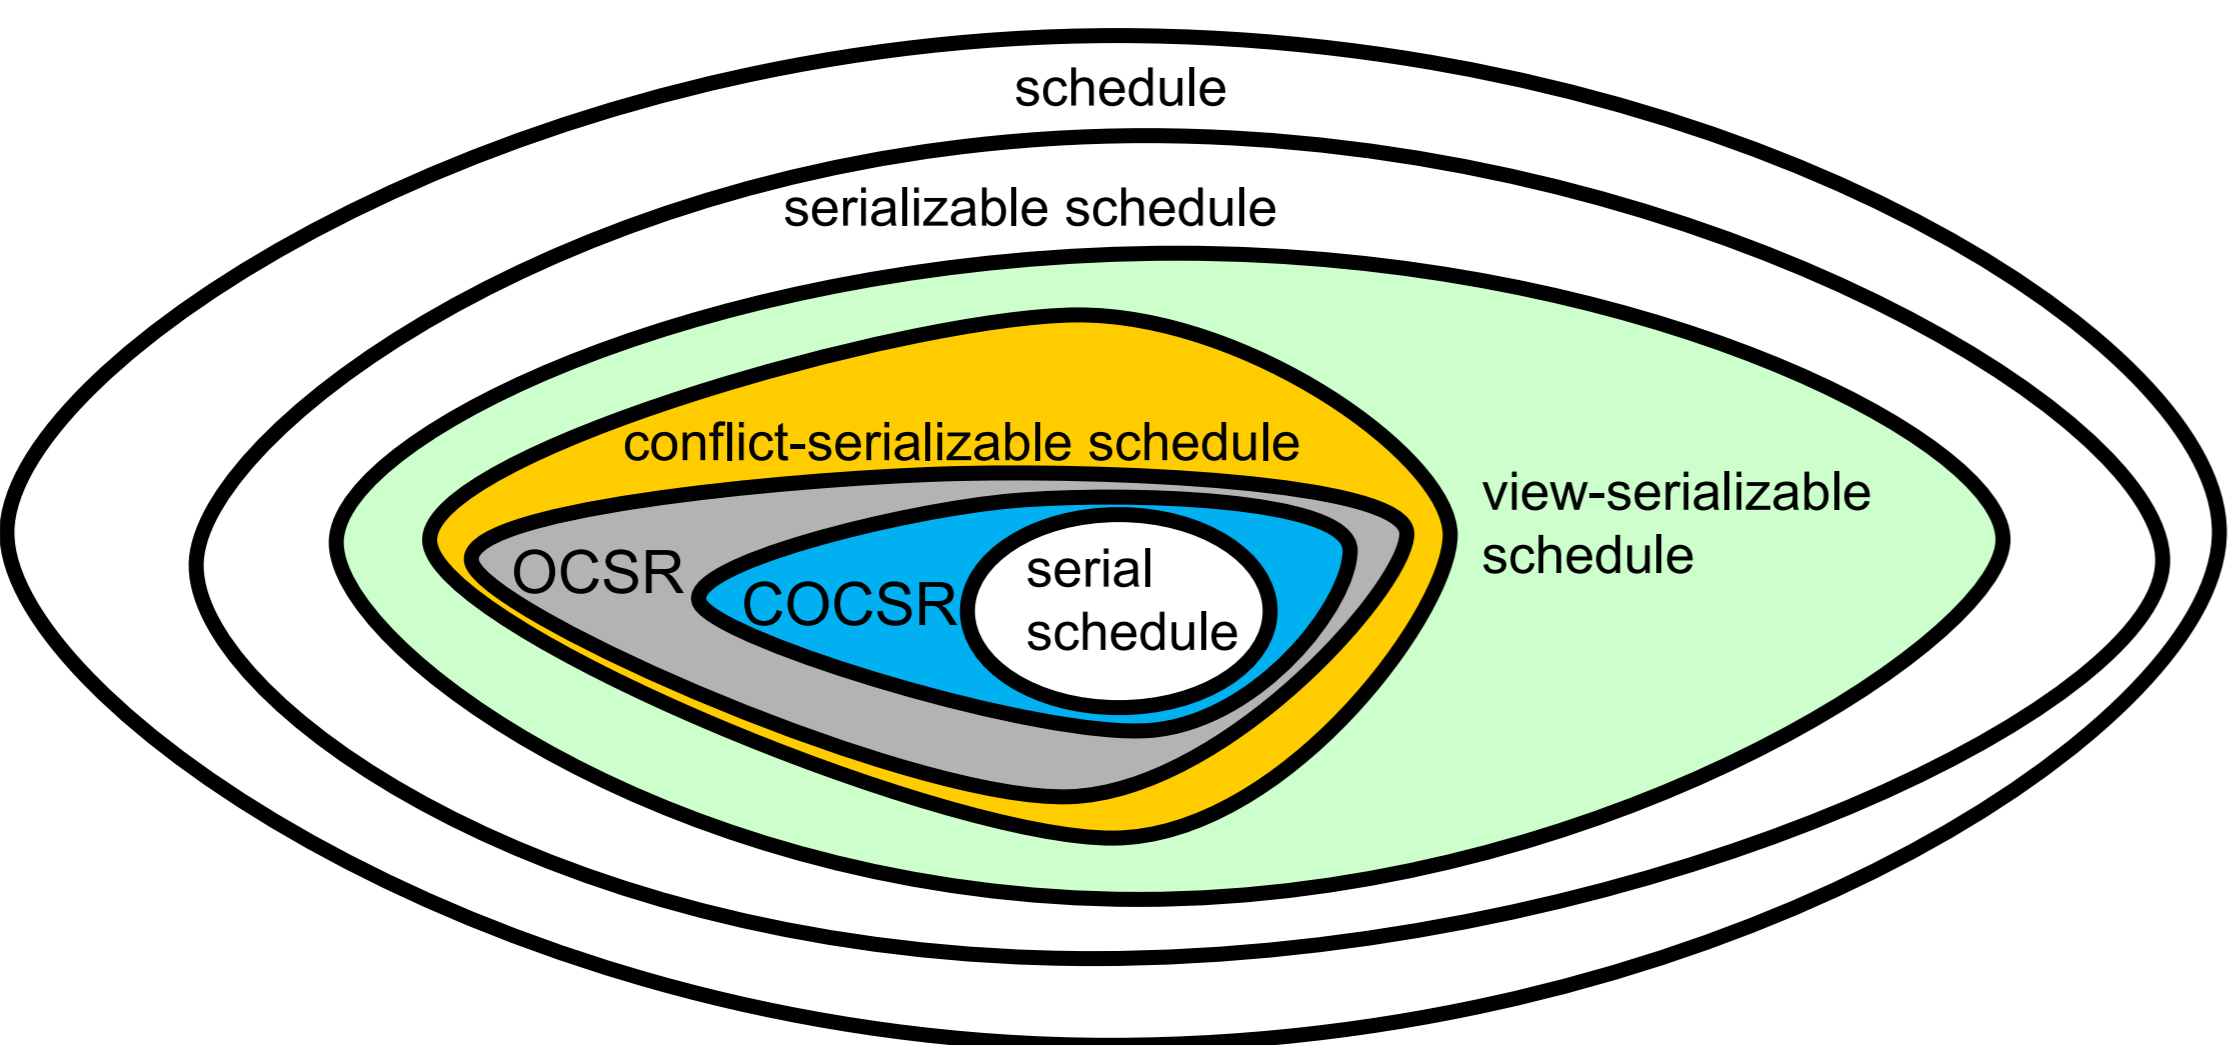
\includegraphics[width=150mm]{aiuto1.png}
\end{figure}
\clearpage
\subsection{Concurrency through locks}
In the methods based on \textbf{locks},\emph{ a transaction} must \emph{ask} and get a \emph{permission} in order to operate of an \emph{element} of the \emph{database}, the \emph{lock} is a mechanism for a transaction to ask and get such a \textbf{permission}. We introduce two new operations used to \emph{request} and \emph{release} the \textbf{exclusive use} of a \emph{resource} (called A), where $i$ stands for the \emph{transaction} $T_i$ that use the operations:
\begin{itemize}
\item \textbf{Lock} (\emph{exclusive}): $l_i(A)$
\item \textbf{Unlock}: $u_i(A)$
\end{itemize}
When we use the \textbf{exclusive locks}, \emph{transactions} and \emph{schedules} should obey \textbf{two rules}: 
\begin{itemize}
\item Every \emph{transaction} is \textbf{well-formed}.
\begin{itemize}
\item A \emph{transaction} $T_i$ is \textbf{well-formed} if every \emph{action} of $T_i$ (\emph{read} or \emph{write} on A) is contained in a \textbf{critical section}, so it delimited by a pair of \textbf{lock-unlock} on A. (\emph{Per ogni azione ce deve sta una coppia di lock-unlock});
\item A \emph{transaction} $T_i$ is \textbf{ill-formed} if it is not \emph{well-formed};
\end{itemize}
\item The \emph{schedule} is \textbf{legal}.
\begin{itemize}
\item A \emph{schedule} $S$ with locks is \textbf{legal} if no transaction in it locks an element A when a different transaction has granted the lock on A and has not yet unlocked A. (\emph{Nessuna transizione deve tocca un elemento se non è ancora stato sbloccato da un altro});
\end{itemize}
\end{itemize}
A \emph{scheduler} based on \textbf{exclusive locks} behaves as follows:
\begin{itemize}
\item When an \textbf{action request} is issued by a \emph{transaction}, the \emph{scheduler} checks whether this \textbf{request} makes the \emph{transaction} \textbf{ill-formed}, in which case the \emph{transaction} is \textbf{aborted} by the scheduler;
\item When a \textbf{lock request} on A is issued by a \emph{transaction} $T_i$ while another transaction has a lock on it, the \emph{scheduler} doesn't grant the request and $T_i$ is \textbf{blocked} until the other transaction \emph{release} the lock on A;
\item To trace all the \emph{locks granted}, the \emph{scheduler} manages a table of the locks called \textbf{lock table};
\end{itemize}
A \emph{schedule} S with \emph{exclusive locks} follows the \textbf{two-phase locking protocol} (\emph{2PL protocol}) if in each \emph{transaction} $T_i$ appearing in S, all \emph{lock operations} \textbf{precede all} \emph{unlock operations}. This \emph{protocol} avoids the \textbf{ghost update} while accepting \emph{concurrency}. In some cases the \emph{scheduler} can \textbf{block} all the \emph{transactions} and none can proceed, this is called \textbf{deadlock}. So we can add a new rule to the scheduler:
\begin{itemize}
\item Every \emph{transaction} is \textbf{well-formed}.
\item The \emph{schedule} is \textbf{legal}.
\item Each \emph{transaction}, extended with the inserted lock/unlock commands, follows the \textbf{2PL protocol}.
\end{itemize}
A \emph{scheduler} based on \textbf{exclusive locks} and \textbf{2PL} behaves as follows (\emph{if the \textbf{lock/unlock} commands are automatically inserted the first two points do not occur}):
\begin{itemize}
\item If a \emph{request} by a \emph{transaction} $T_i$ shows that $T_i$ is not\textbf{ well-formed}, then $T_i$ is \textbf{aborted} by the scheduler;
\item If a \emph{lock request} by a \emph{transition} $T_i$ shows that $T_i$ doesn't follow the \textbf{2PL} then $T_i$ is \textbf{aborted} by the scheduler;
\item If a \textbf{lock} is requested for A by a \emph{transition} $T_i$ while A is used by a different \emph{transition} $T_j$, then the \emph{scheduler} \textbf{blocks} $T_i$  until $T_j$ \emph{release the lock} on A, and if the \emph{scheduler} figures out that a \textbf{deadlock} has occurred or will occur then the \emph{scheduler} adopt a method for \textbf{deadlock management};
\item To trace all the \emph{locks granted}, the \emph{scheduler} manages a table of the locks called \textbf{lock table};
\end{itemize}
\textbf{THEOREM:}
\begin{itemize}
\item Every \emph{legal schedule} constituted by \emph{well-formed} \emph{transactions} following the \emph{2PL protocol} and with \emph{exclusive locks} is \textbf{conflict-serializable}.
\end{itemize}
The theorem says that every \emph{legal schedule} constituted by N \textbf{well-formed} \emph{transactions} following the \emph{2PL protocol} is \textbf{conflict-equivalent} to the \emph{serial schedule} that orders the \emph{transaction} in this order: from 1 to N-1 transition of the schedule takes the \emph{transaction} that execute the first \emph{unlock} operation in the remaining \emph{transaction} in S (so from S, N-1, N-2, ... , to last 2) and at N takes the last \emph{transition} left as the $N^{th}$ \emph{transition} of the \emph{schedule}. \\\\
\textbf{THEOREM:}
\begin{itemize}
\item There exists a \textbf{conflict-serializable schedule} that doesn't follow the \emph{2PL protocol} (with \emph{exclusive locks}). 
\end{itemize}
\begin{figure}[H]
  \centering
  \includegraphics[width=136mm]{cattura3.png}
\end{figure}
\pagebreak
There is a different kind of lock, not restrictive as the \textbf{exclusive lock} (in fact two \emph{read operations} do not create conflict) and it's called \textbf{shared lock}:
\begin{itemize}
\item $sl_i(A)$: \textbf{shared lock};
\item $xl_i(A)$: \textbf{exclusive lock};
\item $u_i(A)$: \textbf{unlock}
\end{itemize}
It is possible to upgrade a \textbf{shared lock} to an \textbf{exclusive lock} on the \emph{same element} by the \emph{same transition} without the \emph{unlock} (of the \emph{shared}) and this is called \textbf{lock upgrade}. With \textbf{shared} and \textbf{exclusive locks} the following rules must be respected:
\begin{itemize}
\item We say that a \emph{transaction} $T_i$ is \textbf{well-formed} if:
\begin{itemize}
\item Every \textbf{read} $r_i(A)$ is preceded by a $sl_i(A)\ or\ by\ xl_i(A)$, with no $u_i(A)$, so every \emph{read operation} is preceded by a \textbf{lock};
\item Every \textbf{write} $w_i(A)$ is preceded by a $xl_i(A)$ with no $u_i(A)$ in between, so every \emph{write operation} is preceded by an \textbf{exclusive lock};
\item Every \textbf{lock} $sl_i(A)\ or\ by\ xl_i(A)$ of a \emph{transaction} $T_i$ is followed by an \textbf{unlock} on A by $T_i$;
\end{itemize}
\item We say that a \emph{schedule S} is \textbf{legal} if:
\begin{itemize}
\item An \textbf{exclusive lock} $xl_i(A)$ is not followed by any other \textbf{lock} $xl_j(A)$ or by any $sl_j(A)$ (from a different transaction $T_j$) without an \textbf{unlock} $u_i(A)$ in between;
\item A \textbf{shared lock} $sl_i(A)$ is not followed by any other \textbf{exclusive lock} $xl_j(A)$ (from a different transaction $T_j$) without an \textbf{unlock} $u_i(A)$ in between;
\end{itemize}
\end{itemize}
With shared locks the \textbf{2PL (two-phase locking) }becomes:
\begin{itemize}
\item A \emph{schedule} $S$ follows the \textbf{2PL protocol} if in every \emph{transaction} $T_i$ of $S$, all \emph{lock operations} (\textbf{exclusive} or \textbf{shared}) precede all \textbf{unlocking} operations of $T_i$;
\item In other words, no \emph{action} $xl_i(X)$ or $sl_i(X)$ can be preceded by an \textbf{unlock} $u_i(Y)$;
\end{itemize}
The scheduler uses the \textbf{compatibility matrix} for deciding whether a \textbf{lock request} should be granted or not. In this matrix $S = shared\ lock, X = exclusive\ lock, YES = request\ granted, NO = request\ not\ granted$.
\begin{figure}[H]
  \centering
  \includegraphics[width=140mm]{cattura4.png}
\end{figure}
\clearpage 
The problem for the \emph{scheduler} of automatically inserting the \textbf{lock/unlock commands} becomes more complex in the presence of \emph{shared locks}, and also the execution of the \textbf{unlock commands} requires more work, in fact when an \emph{unlock} is issued there may be several \emph{transaction} waiting for a \emph{lock} (\emph{exclusive} or \emph{shared}) and the \emph{scheduler} must \textbf{decide} to which \emph{transaction} grant the \emph{lock} and there are several methods:
\begin{itemize}
\item \textbf{First-come-first-served};
\item Give priorities to the \emph{transaction} asking for a \textbf{shared lock};
\item Give priorities to the \emph{transaction} asking for a \textbf{exclusive lock}
\end{itemize}
The \textbf{FCFS} is the most used one cause it avoids \textbf{starvation}, that is the situation in which a \emph{request} of a \emph{transaction} is never granted. The properties of two-phase locking with shared and exclusive locks are similar to the case of exclusive locks only:\\\\
\textbf{THEOREM:}
\begin{itemize}
\item Every \emph{legal schedule} constituted by \emph{well-formed} \emph{transactions} following the \emph{2PL protocol} and with \emph{exclusive locks and shared locks} is \textbf{conflict-serializable}.
\end{itemize}
\textbf{THEOREM:}
\begin{itemize}
\item There exists a \textbf{conflict-serializable schedule} that doesn't follow the \emph{2PL protocol} (with \emph{exclusive locks and shared locks}). 
\end{itemize}
\begin{figure}[H]
  \centering
  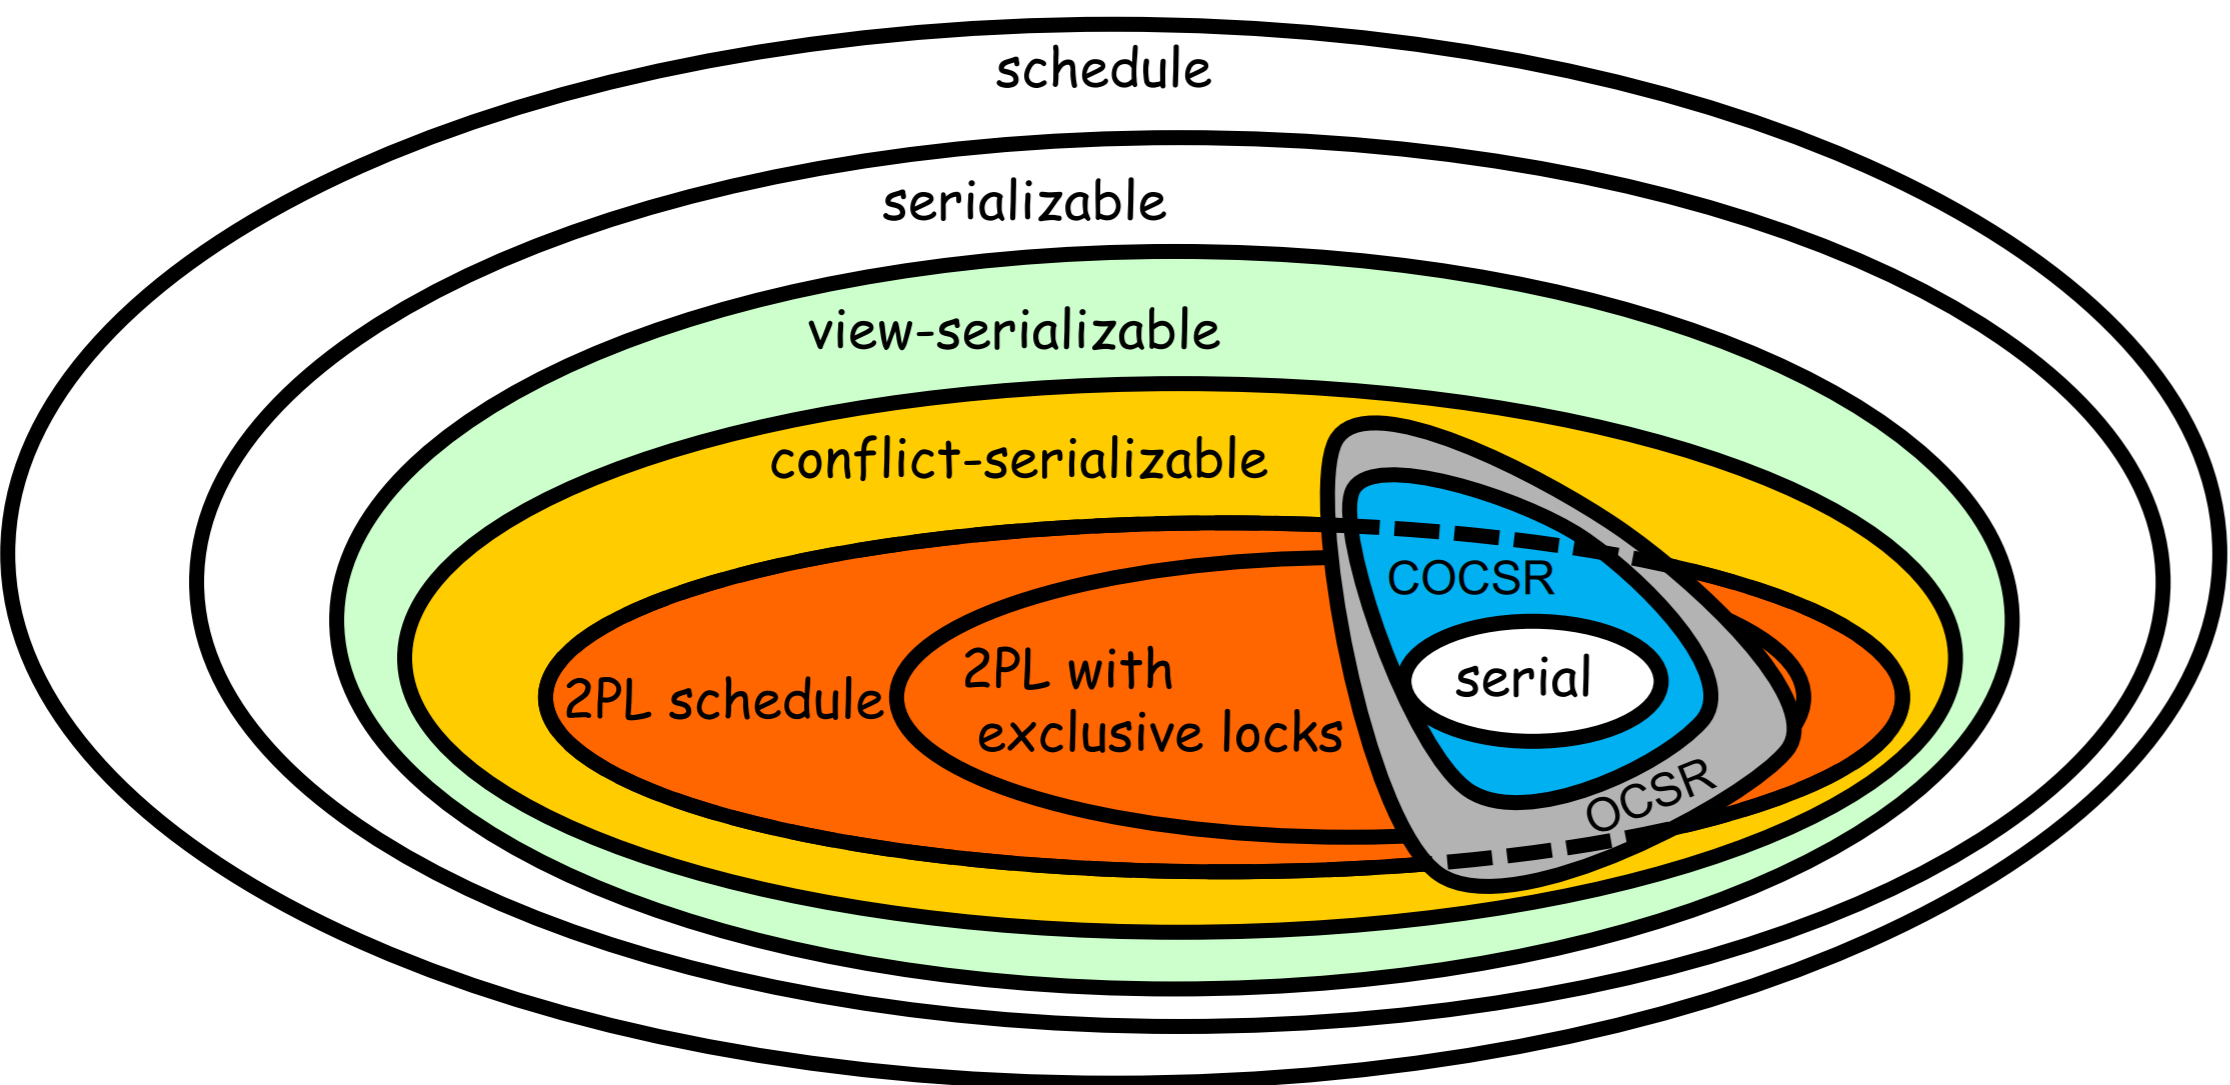
\includegraphics[width=116mm]{cattura5.png}
\end{figure}
Even with \textbf{shared locks} the risk of \textbf{deadlock}(two \emph{transaction} need an \emph{exclusive lock} on the element used by the other, so none proceed) is still present for example in: $sl_1(A), sl_2(A), xl_1(A), xl_2(A)$. The probability of a \emph{deadlock} grows \textbf{linearly} with the \emph{number of transactions} and \textbf{quadratically} with the \emph{number of} \emph{lock requests} in the \emph{transactions}. 
\clearpage
There are several techniques for \textbf{deadlock management}:
\begin{itemize}
\item \textbf{Timeout};
\begin{itemize}
\item The system fixes a \textbf{timeout} $t$ after which a \emph{transaction} waiting for a \emph{lock} is \textbf{killed}. It is a very simple technique, but it $t$ is \emph{high}, the risk to be late in solving the problem, instead if $t$ is \emph{low}, too many \emph{transaction} are \emph{killed}. And there is another problem, the risk of \textbf{individual block} (the same transaction is killed several times);
\end{itemize}
\item \textbf{Deadlock recognition};
\begin{itemize}
\item A \textbf{wait-for graph} is incrementally maintained: the \textbf{nodes} are the \emph{transactions}, and the \textbf{edge} ($T_i,T_j$) means that $T_i$ is waiting for $T_j$ to release a \emph{lock}. When a \emph{cycle} appears in the graph, that means that there is a \textbf{deadlock}, and it's resolved by killing one of the involved \emph{transactions};
\end{itemize}
\item \textbf{Deadlock prevention};
\begin{itemize}
\item Also called \textbf{wait-die}, in which to each \emph{transaction} $T_i$ a \textbf{priority} $pr(T_i)$ is assigned, in such a way that different \emph{transactions} have different \emph{priorities}, and the rule is: in case of conflict on a \emph{lock}, $T_i$ is allowed to wait $T_j$ only if $pr(T_i) > pr(T_j)$ otherwise the \emph{transaction} $T_i$ is killed. In practice when a new \emph{edge} ($T_i,T_j$) is added in the \textbf{wait-for} graph if $pr(T_i) \leq pr(T_j)$ then $T_i$ is killed;
\end{itemize}
\end{itemize}
\subsection{Recoverability of transactions}
So far, we study under the assumption that no \emph{transaction} are \textbf{rollbacked}. In fact, with \textbf{rollbacks} the notion of \emph{serializability} that we have considered up to now is not sufficient for achieving the \textbf{ACID properties}. This fact is testified by an anomaly called \textbf{dirty read}, a \textbf{WR anomaly}. Let's consider two transactions $T_1$ and $T_2$ both with the same commands:\\

\InsertBoxL{0}{\includegraphics[scale=0.35]{cattura6.png}}% 
\[READ(A,x) ,\ x := x + 1 ,\ WRITE(A,x)\]
Let's consider the following \emph{schedule} (where $T_1$ executes the \textbf{rollback}), the problem is that $T_2$ reads a \emph{value} written by $T_1$ before $T_1$ \textbf{commits} or \textbf{rollback}, so, $T_2$ reads a \textbf{dirty value}, that is shown to be \emph{incorrect} when the \emph{rollback} of $T_1$ is executed. The behavior of $T_2$ depends on a \emph{incorrect input value}.%
\\\\Recall that, at the end of \emph{transaction} $T_i$:
\begin{itemize}
\item If $T_i$ has executed the \textbf{commit operation}:
\begin{itemize}
\item The \emph{system} should ensure that the effects of the \emph{transaction} are \textbf{recorded permanently} in the \emph{database};
\end{itemize}
\item If $T_i$ has executed the \textbf{rollback operation}:
\begin{itemize}
\item The \emph{system} should ensure that the effect of the \emph{transaction} has \textbf{no effect} on the \emph{database};
\end{itemize}
\end{itemize}
\clearpage
It's important to note that the \textbf{rollback} of a \emph{transaction} $T_i$ can trigger the \emph{rollback} of other \emph{transactions}, in a \textbf{cascading mode}. In fact if a transaction $T_j$ has read from $T_i$, we should kill $T_j$, and if another $T_k$ has read from $T_j$...	This is called \textbf{cascading rollback} and should be avoided cause it causes several \emph{performance problems}. 
\subsubsection{Recoverable schedules}
A schedule is \textbf{recoverable} if no \emph{transaction} in S \emph{commits} before all other \emph{transaction} it has \textbf{read from}, \emph{commit}. \textbf{Serializability} and \textbf{recoverabilty} are two orthogonal concepts, in fact there are \emph{recoverable schedules} that are \emph{non-serializable} and \emph{serializable schedule} that are not \emph{recoverable}. Every \textbf{serial schedule} is \textbf{recoverable}. In other words:
\begin{itemize}
\item S is \textbf{recoverable} if no \emph{transaction} in S \emph{commits} before the \emph{commit} of all the \emph{transactions} it has\textbf{ read from}, \emph{example}:
\[w_1(A)\ w_1(B)\ w_2(A)\ r_2(B)\ c_1\ c_2\]
\item \emph{Ogni transizione committa dopo di tutte le transizioni da cui ha letto (?)}.
\end{itemize}
\subsubsection{ACR schedules}
\textbf{Recoverable schedules} can still suffer from the \textbf{cascading rollback problem}, and to avoid it, we need a stronger condition:
\begin{itemize}
\item A \emph{schedule} S avoids \emph{cascading rollback} (the schedule is \textbf{ACR}) if every \emph{transactions} in S \emph{reads} values that are \emph{written} by \emph{transactions} that have already \textbf{committed}, so an ACR schedule blocks the dirty data anomaly;
\item S is \textbf{ACR} if no \emph{transaction} \textbf{reads from} a \emph{transaction} that has not \emph{committed} yet, \emph{example}:
\[w_1(A)\ w_1(B)\ w_2(A)\ c_1\ r_2(B)\ c_2\]
\item Not all \emph{\textbf{ACR} schedules} are \textbf{serializable}, and every \textbf{ACR} is \textbf{recoverable} and every \emph{serial schedule} is \textbf{ACR}.
\item So every \emph{ACR schedules} blocks the \textbf{WR} \emph{dirty read anomaly};
\end{itemize}
\subsubsection{Strict schedules}
In a \emph{schedule} S, we say that a \emph{transaction} $T_i$ \textbf{writes on} $T_j$ if there is a $w_j(A)$ in S followed by $w_i(A)$ and there is no \emph{write} operations on A in S between these two \emph{actions}.
\begin{itemize}
\item A \emph{schedule} S is \textbf{strict} if every \emph{transaction} \textbf{reads only} values written by \emph{transactions} that have already \emph{committed}, and \textbf{writes only} on \emph{transactions} that have already \emph{committed};
\item So, every \textbf{strict} schedule is ACR and when a transaction $T_i$ rollbacks, it's immediate to determine which are the values that have to be stored back in the database to reflect the rollback of $T_i$, cause no transaction may have written on this values after $T_i$;
\item Every \emph{serial schedule} is \textbf{strict}, and every \textbf{strict} is \emph{ACR} and so \emph{recoverable}, but not all \textbf{ACR} \emph{schedules} are \emph{strict};
\item So every \emph{strict schedules} blocks \textbf{WR} and \textbf{WW} operations;
\end{itemize}
\subsubsection{Rigorous schedules}
\begin{itemize}
\item A \emph{schedule} is \textbf{rigorous} if for each pair of \textbf{conflicting actions} $a_i$ (of $T_i$) and $b_j$ (of $T_j$) appearing in S, the \emph{commit} command $c_i$ of $T_i$ appears in S between $a_i$ and $b_j$;
\item Every \emph{serial schedule} is \textbf{rigorous} and every \textbf{rigorous} is \emph{strict}, and therefor \emph{ACR} and \emph{recoverable}, but not all \emph{strict schedules} are \emph{rigorous};
\end{itemize}
\begin{figure}[H]
  \centering
  \includegraphics[width=80mm]{cattura7.png}
\end{figure}
\subsubsection{Strict 2PL}
A \emph{schedule} S is said to be in the \textbf{strict 2PL} if  S is in \textbf{2PL} and S is \textbf{strict};
\begin{itemize}
\item  A \emph{schedule} S follows the \textbf{strict 2PL protocol} (S2PL) if it follows the \emph{2PL protocol}, and all \textbf{exclusive locks} of every \emph{transaction} T are kept by T until either T \emph{commits} or \emph{rollbacks}. 
\begin{itemize}
\item Every \emph{schedule} following this protocol is \textbf{strict} and \emph{serializable}. 
\end{itemize}
\item A \emph{schedule} S follows the \textbf{strong strict 2PL protocol} (SS2PL) if it follows the \emph{2PL protocol}, and all \textbf{locks} of every \emph{transaction} T are kept by T until either T \emph{commits} or \emph{rollbacks}. 
\begin{itemize}
\item Every \emph{schedule} S following this protocol is \textbf{rigorous}, \emph{serializable} and the commit order of S is also a \emph{conflict-serializablity order;}
\end{itemize}
\end{itemize}
\begin{figure}[H]
  \centering
  \includegraphics[width=116mm]{cattura8.png}
\end{figure}
\subsection{Concurrency through timestamps}
Each \emph{transition} $T$ has an associated \textbf{timestamp} $ts(T)$ that is unique among the \emph{active transactions} and is such that $ts(T_i) < ts(T_j)$ whenever a \emph{transaction} $T_i$ arrives at \emph{scheduler} before $T_j$. So, the timestamps actually define a total order on transactions. Every \emph{schedule} respecting the \textbf{timestamp order} is \textbf{conflict-serializable} cause it's \emph{conflict-equivalent} to the \emph{serial schedule} corresponding to the \emph{timestamp order}. The use of \emph{timestamps} avoids the use of \emph{locks}, but the \textbf{deadlock} may still occur. The basic idea is that at each action execution, the \emph{schedules} checks whether the involved \emph{timestamps} violates the \textbf{serializablity} condition according to the \emph{order} induced by the \emph{timestamps}. In particular for each element X we maintain the following data:
\begin{itemize}
\item \emph{rts(X)}: the \emph{highest timestamp} among the \emph{active transactions} that have \textbf{read} X;
\item \emph{wts(X)}: the \emph{highest timestamp} among the \emph{active transactions} that have \textbf{written} X 
\item \emph{wts-c(X)}: the \emph{timestamp} of the last \emph{committed transaction }that has \textbf{written} X;
\item \emph{cb(X)}: a bit called \textbf{commit-bit }that is \emph{false} if the last transaction that \textbf{wrote} X has not \emph{committed} yet, or \emph{true} otherwise;
\end{itemize}
The rules are:
\begin{itemize}
\item The \emph{actions} of \emph{transaction} $T$ is a \emph{schedule} $S$ must be considered as being \textbf{logically executed} in \emph{one spot};
\item The \textbf{logical time} of an \emph{action} of $T$, is the \textbf{timestamp} of $T$, $ts(T)$;
\item The \emph{commit-bit} is used in order to avoid the \textbf{dirty-read anomaly};
\item We assume that the \textbf{timestamp} so the \textbf{logical time} of each \emph{transaction} coincide with the subscript: $ts(T_i) = i$, instead the \textbf{physical time} will be denoted as $t_1, ... , t_n$;
\end{itemize}
The system manages two \emph{temporal axes}, the \textbf{physical time} and the \textbf{logical time}. The values of \emph{rts(X)} and \emph{wts(X)} indicate the \emph{timestamp} of the \emph{transaction} that was the last to \emph{read} and \emph{write} on X according to the \emph{logical time}. An action of a \emph{transaction} $T$ executed at the \textbf{physical time} $t$ is \emph{accepted} if its \emph{ordering} according to the \emph{physical temporal} order is compatible with respect to the \textbf{logical time}: $ts(T)$. This principle of compatibility is checked by the \emph{scheduler}.
\subsubsection {Case 1a - Read ok}
\begin{figure}[H]
  \centering
  \includegraphics[width=116mm]{cattura9.png}
\end{figure}
Consider $r_2(X)$ with respect to the \textbf{last} \textbf{write} on X, $w_1(X)$:
\begin{itemize}
\item The \textbf{physical time} of $r_2(X)$ is $t_6$ that is \emph{greater} than the \emph{physical time} of $w_1(X)$ that is $t_4$;
\item The \textbf{logical time} of $r_2(X)$ is $ts(T_2)$ that is \emph{greater} than the \emph{logical time }of $w_1(X)$ that is $wts(X) = ts(T_1)$;
\end{itemize}
So there is \textbf{no incompatibility} between \emph{logical} and \emph{physical time}, so we proceed as follows:
\begin{itemize}
\item If $cb(X)$ is \emph{true}, so if $T_1$ \textbf{committed}, the $rts(X)$ should be to the \textbf{maximum} between $rts(X)$ and $ts(T)$, in this example $rts(X) = ts(T_3)$ cause $ts(T_3)$ of operation $r_3(X)$ is greater than $ts(T_2)$ of operation $r_2(X)$, so $r_2(X)$ is executed and the schedules goes on;
\item If $cb(X)$ is \emph{false}, then $T_2$ is put in a \textbf{waiting state} for the \emph{commit} or the \emph{rollback} of the \emph{transaction} that was the last to \emph{write} X;
\end{itemize}
\subsubsection {Case 1b - Read too late}
\begin{figure}[H]
  \centering
  \includegraphics[width=116mm]{cattura10.png}
\end{figure}
Consider $r_1(X)$ with respect to the \textbf{last} \textbf{write} on X, $w_2(X)$:
\begin{itemize}
\item The \textbf{physical time} of $r_1(X)$ is $t_4$ that is \emph{greater} than the \emph{physical time} of $w_2(X)$ that is $t_3$;
\item The \textbf{logical time} of $r_1(X)$ is $ts(T_1)$ that is \emph{less} than the \emph{logical time} of $w_2(X)$ that is $wts(X) = ts(T_2)$;
\end{itemize}
So there is \textbf{incompatibility}, and the action of $r_1(X)\ of\ T_1$ cannot be executed, so $T_1$ \emph{rollbacks} and a new execution of $T_1$ starts with a new \emph{timestamp}. 
\subsubsection {Case 2a - Write ok}
\begin{figure}[H]
  \centering
  \includegraphics[width=116mm]{cattura11.png}
\end{figure}
Consider $w_3(X)$ with respect to the \textbf{last read} on X, $r_1(X)$, and the \textbf{last write} on X, $w_2(X)$:
\begin{itemize}
\item The \textbf{physical time} of $w_3(X)$ is $t_6$ that is \emph{greater} than the \emph{physical time} of $r_1(X)$ and $w_2(X)$ ($t_4\ and\ t_5$);
\item The \textbf{logical time} of $w_3(X)$ is $t_6$ that is \emph{greater} than the \emph{logical time} of $r_1(X)$ and $w_2(X)$;
\end{itemize}
So there is \textbf{no incompatibility} between \emph{logical} and \emph{physical time}, so we proceed as follows:
\begin{itemize}
\item If $cb(X)$ is \emph{true} and \textbf{no active transaction wrote} X: we set $wts(X) = ts(T_3)$, we set $cb(X) = false$ and the action $w_3(X)\ of\ T_3$ is executed and the \emph{schedule} goes on;
\item If $cb(X)$ is \emph{false}, then $T_3$ is put in a \textbf{waiting state} for the \emph{commit} or the \emph{rollback} of the \emph{transaction} that was the last to \emph{write} X;
\end{itemize}
\subsubsection {Case 2b - Thomas Rule}
\begin{figure}[H]
  \centering
  \includegraphics[width=116mm]{cattura12.png}
\end{figure}
Consider $w_1(X)$ with respect to the \textbf{last read} $r_1(X)$ on X:
\begin{itemize}
\item The \textbf{physical time} of $w_1(X)$ is $t_6$ that is \emph{greater} than the \emph{physical time} of $r_1(X)$, $t_4$;
\item The \textbf{logical time} is \emph{equal} cause the two operations belongs to the same \emph{transaction};
\end{itemize}
So there is \textbf{no incompatibility} between \emph{logical} and \emph{physical time}, but on the \textbf{logical time dimension} $w_2(X)$ comes after the write $w_1(X)$ so the execution of $w_1(X)$ would correspond to an \textbf{update loss}. Therefor:
\begin{itemize}
\item If $cb(X)$ is \emph{true}, we simply ignore $w_1(X)$ (not executed), in this way the effect is to \emph{correctly} \textbf{overwrite} the value \emph{written} by $T_1$ on X, with the value written by $T_2$ on X, so we pretend that $w_1(X)$ came before $w_2(X)$;
\item If $cb(X)$ is \emph{false}, then $T_1$ is put in a \textbf{waiting state} for the \emph{commit} or the \emph{rollback} of the \emph{transaction} that was the last to \emph{write} X;
\end{itemize}
\subsubsection {Case 2c - Write too late}
\begin{figure}[H]
  \centering
  \includegraphics[width=116mm]{cattura13.png}
\end{figure}
Consider $w_1(X)$ with respect to the \textbf{last read} $r_2(X)$ on X:
\begin{itemize}
\item The \textbf{physical time} of $w_1(X)$ is $t_4$ that is \emph{greater} than the \emph{physical time} of $r_2(X)$, $t_3$;
\item The \textbf{logical time} of $w_1(X)$ is $ts(T_1)$ that is \emph{less} than the \emph{logical time} of $r_2(X)$, $rts(X) = ts(T_2)$;
\end{itemize}
So there is \textbf{incompatibility}, and the action of $w_1(X)\ of\ T_1$ cannot be executed, so $T_1$ is \textbf{aborted}, and a new execution of $T_1$ starts with a new timestamp.
\subsubsection{Deadlock with timestamps}
The methods of \emph{timestamps} doesn't avoid the risk of \textbf{deadlock}, but the probability is \emph{lower} than in the case of \emph{locks}. The \emph{deadlock} is related to the use of the\textbf{ commit-bit}, and the \textbf{deadlock problem} is handled with the same techniques used in \emph{2PL method}.
\subsubsection{Conflict-serializability and timestamps}
There are \textbf{conflict-serializable} \emph{schedules} that are not accepted by the \emph{timestamp-based scheduler}. 
\begin{itemize}
\item If the \emph{schedule} S is \emph{processed} by the \textbf{timestamp-based scheduler} without using the \textbf{Thomas rule}, then the schedule obtained from S by removing all \emph{actions} of \emph{rollbacked transaction} is \textbf{conflict-serializable};
\item If the \emph{schedule} S is \emph{accepted} by the \textbf{timestamp-based scheduler} using the \textbf{Thomas rule}, then S may be not \textbf{conflict-serializable};
\item If the \emph{schedule} S is \emph{accepted} by the \textbf{timestamp-based scheduler} using the \textbf{Thomas rule}, then the \emph{schedule} obtained from S by removing all \emph{actions} ignored by the \emph{Thomas rule} and all \emph{actions} of \emph{rollbacked transaction} is \textbf{conflict-serializable};
\end{itemize}
\subsubsection{Timestamps and 2PL}
\begin{itemize}
\item There are \emph{schedules} that are accepted by \emph{timestamp-based schedulers} that are \textbf{not in 2PL};
\item There are \emph{schedules} that are accepted by \emph{timestamp-based schedulers} and are also \textbf{strict 2PL};
\item There are \textbf{strong strict 2PL schedules} that are not accepted by \emph{timestamp-based scheduler};
\end{itemize}
\begin{figure}[H]
  \centering
  \includegraphics[width=116mm]{cattura14.png}
   \caption{All types of schedules including timestamp}
\end{figure}
\begin{figure}[H]
  \centering
  \includegraphics[width=146mm]{cattura15.png}
   \caption{Comparison between Timestamps and 2PL}
\end{figure}
\subsubsection{Multiversion timestamp}
The idea is to \textbf{don't block the \emph{read action}}, and this is made by introducing \emph{different version} of an element $X$: $X_1, ... , X_n$, so that every \emph{read} can be always be executed, provided that the right version is chosen (according to the \emph{logical time} determined by the \emph{timestamp}):
\begin{itemize}
\item Every \textbf{legal write} $w_i(X)$ generates a \textbf{new version} $X_i$;
\item To \emph{each version} $X_h$ of $X$ the \emph{timestamp} $wts(X_h) = ts(T_h)$ is \emph{associated}, denoting the \textbf{timestamp} of the transaction that \textbf{wrote} that version;
\item To \emph{each} \emph{version} $X_h$ of $X$ the \emph{timestamp} $rts(X_h) = ts(T_h)$ is \emph{associated}, denoting the \textbf{highest timestamp} among those \emph{transactions} that \textbf{read} $X_h$;
\end{itemize}
The \emph{scheduler} uses \textbf{timestamps} as follows:
\begin{itemize}
\item When executing $w_i(X)$, if a \emph{read} $r_j(X_k)$ such that $wts(X_k) < ts(T_i) < ts(T_j)$ already occurred, then the \textbf{write is refused} (cause a $T_j$ older than $T_i$ has already \emph{read} a version of X that precedes $X_i$), otherwise the \textbf{write is executed} on a new version $X_i$ of $X$ and $wts(X_i) = ts(T_i)$;
\item When executing a $r_i(X)$, the \emph{read} is executed on the \emph{version} $X_j$ such that $wts(X_j)$ is the \textbf{highest write timestamp} among the versions of X, and \textbf{less or equal} to $ts(T_i)$, so $wts(X_j) \leq ts(T_i)$ and there is no version $X_h$ such that $wts(X_j) < wts(X_h) \leq ts(T_i)$;
\item For $X_j$ with $wts(X_j)$ such that \textbf{no active transaction} has \emph{timestamp} \textbf{less} than $j$, the version of $X$ that precede $X_j$ are deleted from \emph{oldest} to \emph{newest};
\item To ensure \emph{recoverability}, the commit of $T_i$ is delayed until all \emph{commits} of the \emph{transactions} $T_j$ that \emph{wrote} versions \emph{read} by $T_i$ are executed;
\end{itemize}
The \emph{scheduler} uses suitable \textbf{data structures};
\begin{itemize}
\item For each version $X_i$ the \emph{scheduler} maintains a $range(X_i) = [wts, rts]$ where \textbf{wts} is the \emph{timestamp} of the \emph{transaction} that \emph{wrote} $X_i$, and \textbf{rts} is the \emph{highest timestamp} among those of the \emph{transaction} that \emph{read} $X_i$ (if none, $rts=wts$);
\item We denote the \emph{set}: $ranges(X) = \left \{ range(X_i)\ |\ X_i\ is\ a\ version\ of\ X \right \}$
\item When $r_i(X)$ is processed, the \emph{scheduler} uses the set $ranges(X)$ to find the version $X_j$ such that $range(X_j) = [wts, rts]$ where \textbf{wts} is the highest, and less or equal to the \emph{timestamp} of $T_i$, and if $ts(T_i) > rts$ then the $rts$ of $range(X_j)$ is set to $ts(T_i)$;
\item When $w_i(X)$ is processed, the \emph{scheduler} uses the set $ranges(X)$ to find the version $X_j$ such that $range(X_j) = [wts, rts]$ where \textbf{wts} is the highest, and less or equal to the \emph{timestamp} of $T_i$, and if $rts > ts(T_i)$, then $w_i(X)$ is \textbf{rejected}, else is \textbf{accepted} and the version $X_i$ with $range(X_i) = [wts,rts]$ with $wts = rts = ts(T_i)$ is \textbf{created};
\end{itemize}
\section{Cap 4: Recovery}
The \textbf{transaction manager} is mainly concerned with \emph{isolation} and \emph{consistency}, while the \textbf{recovery manager} is mainly concerned with \emph{atomicity} and \emph{persistency}. In fact the recovery manager is responsible for:
\begin{itemize}
\item \textbf{Beginning} the execution of \emph{transactions};
\item \textbf{Committing} \emph{transactions};
\item Executing the \textbf{rollback} of \emph{transactions};
\item Restore a \textbf{correct state }of the \emph{database} following a \emph{fault condition};
\end{itemize}
It use a special \emph{data structure} called \textbf{log file}. \textbf{Failures} can be of two types: 
\begin{itemize}
\item \textbf{System failures}: system crash, system error or application exception, local error condition of a transaction, concurrency control;
\item \textbf{Storage media failures}: disk failures, catastrophic events;
\end{itemize}
The \textbf{log file} records the \emph{actions} of the various \emph{transactions} in a \textbf{stable storage} (\emph{failure resistant storage}). \emph{Read} and \emph{write} operations on the \textbf{log} are executed as the \emph{operations} on the \emph{database} (on the \emph{buffer}), and writing on the \emph{stable storage} is done generally with \emph{force operation}. Of course \emph{stable storage} is an \textbf{abstraction}, in fact \emph{stability} is achieved through \textbf{replication}. The \textbf{log} is a \emph{sequential file }assumed to be \emph{failure-free}. The operations on the \emph{log} are:
\begin{itemize}
\item \textbf{Append a record} at the end;
\item \textbf{Scan sequentially forward};
\item \textbf{Scan backward};
\end{itemize}
The \emph{log} records the \emph{actions} of the \emph{transactions} in \textbf{chronologically order}, and there are two types of records in the \emph{log}:
\begin{itemize}
\item \textbf{Transaction records} (\emph{begin, insert, delete, update, commit, abort});
\item \textbf{System records} (\emph{checkpoint, dump}); 
\end{itemize} 
It's important to not confuse \textbf{transaction actions} with the \textbf{actions on the secondary storage}, in fact the \emph{actions} of the \emph{transaction} are executed when they are recorded in the \emph{log} even if their effects are not yet registered in the \emph{secondary storage}.
\subsection{Transaction Records}
\begin{itemize}
\item \textbf{O} = Element of the database;
\item \textbf{AS} = After State, value of O after an operation;
\item \textbf{BS} = Before State, value of O before an operation;
\end{itemize}
\pagebreak
For each \emph{transaction} T, the \textbf{transaction records} are stored in the \textbf{log} as follows;
\begin{itemize}
\item \textbf{Begin}: $B(T)$;
\item \textbf{Insert}: $I(T,O,AS)$;
\item \textbf{Delete}: $D(T,O,BS)$;
\item \textbf{Update}: $U(T,O,BS,AS)$;
\item \textbf{Commit}: $C(T)$;
\item \textbf{Abort}: $A(T)$;
\end{itemize}
\subsection{System Records}
\subsubsection{Checkpoint}
The goal of the \textbf{checkpoint} is to register in the \emph{log} the set of \textbf{active transaction} $T_1, ..., T_n$, so as to \emph{differentiate} them from the \textbf{committed transactions}. The \textbf{checkpoint} $CK$ operation executes the following \emph{actions}:
\begin{itemize}
\item For each \emph{committed transaction} after the last \emph{checkpoint}, their \textbf{buffer pages} are copied into the \emph{secondary storage} through \textbf{flush};
\item A \emph{record} $CK(T_1, ..., T_n)$ is written on the \textbf{log} through \textbf{force}, where $T_1, ... , T_n$ are all \emph{active transactions} \textbf{uncommitted};
\end{itemize}
It follows that, for each \emph{transaction} $T$ such that $Commit(T)$ precedes $CK(T_1, ..., T_n)$ in the log we can avoid the \textbf{redo} in case of \emph{failure}. This operation is executed \emph{periodically} with \textbf{fixed frequency}.
\subsubsection{Dump}
The \textbf{dump} is a copy of the \textbf{entire state of the database}, and is executed \emph{offline} (so all the \emph{transactions} are suspended). It produces a \textbf{backup}, that is saved in a \emph{stable storage}. This operation write through \emph{flush} a \emph{dump record }in the \emph{log}. 
\subsection{Undo and Redo operations}
\begin{itemize}
\item The\textbf{ undo operation} restore the \emph{state} of an \emph{element} O at the \textbf{time preceding} the execution of an \emph{action};
\item The \textbf{redo operation} restore the \emph{state} of an \emph{element} O at the \textbf{time following} the execution of an \emph{action};
\end{itemize}
The outcome of a \emph{transaction} is established when either the $\mathbf{Commit(T)}$ record or the $\mathbf{Abort(T)}$ record is written in the \textbf{log}. The $Commit(T)$ is written \emph{synchronously} from the \emph{buffer} to the \emph{log}, while the $Abort(T)$ is written \emph{asynchronously}. when a \textbf{failure} occurs for a \emph{transaction} that is \textbf{uncommitted} we need to \textbf{undo} the \emph{actions} to ensure \emph{atomicity}, instead if is \textbf{committed}, we need to \textbf{redo} the \emph{actions} to ensure \emph{durability}.
\subsection {Writing records in the log}
The \textbf{recovery manager} follows two \emph{rules}:
\begin{itemize}
\item \textbf{WAL} or \textbf{write-ahead log}:
\begin{itemize}
\item The \emph{log records} are written from the \textbf{buffer} to the \textbf{log} before the \textbf{corresponding records} are \emph{written} in the \emph{secondary storage};
\item This is important for the \emph{effectiveness} of the \textbf{Undo operation}, cause the old values can always be \emph{written back} to the \emph{secondary storage} by using the \emph{BS value}. In other words, \textbf{WAL} allows to \textbf{undo write operation} executed by \emph{uncommitted} \emph{transaction};
\end{itemize}
\item \textbf{Commit-Precedence}:
\begin{itemize}
\item The \emph{log records} are written from the \textbf{buffer} to the \textbf{log} before the \emph{commit} of the \emph{transaction};
\item This is important for the \emph{effectiveness} of the \textbf{Redo operation}, cause if a \emph{transaction} committed before a \emph{failure}, but its \emph{pages} have not been written yet in \emph{secondary storage} we can use \emph{AS value} to \textbf{write} such pages. In other words, \textbf{Commit-Precedence} allows \emph{committed transactions} whose \emph{effect} have not been registered yet in the \emph{database} to be \textbf{redone}. 
\end{itemize}
\end{itemize}
\subsection{Writing records in secondary storage}
For each operation of \textbf{Update, Insert, Delete}, the \emph{recovery manager} must decide on the strategy for \emph{writing} in the \emph{secondary storage}, and there are three possible methods, all coherent with the \textbf{WAL} and the \textbf{Commit-Precedence} rules:
\begin{itemize}
\item \textbf{Immediate effect}:
\begin{itemize}
\item The \textbf{update operations} are executed \emph{immediately} on the \emph{secondary storage} after the \emph{corresponding records} are \emph{written} in the \emph{log};
\item The \emph{buffer manager writes} the effect of an operation by a \emph{transaction} $T$ on the \emph{secondary storage} \textbf{before} \emph{writing} the \textbf{commit record} of T in \emph{log};
\item So all pages of the \emph{database} modified by a \emph{transaction} are certainly written in the \emph{secondary storage}, and \textbf{Redo is not needed;}
\end{itemize}
\item \textbf{Delayed effect}:
\begin{itemize}
\item The \textbf{update operations} by a \emph{transaction} $T$ are executed on the \emph{secondary storage} only after the \emph{commit} of the \emph{transaction}, so only after the \emph{commit record} of T has been written in the \emph{log}, and \textbf{Undo is not needed};
\item The \textbf{log records} are \emph{written} in the \emph{log} before the \emph{corresponding data} are \emph{written} in \emph{secondary storage};
\end{itemize}
\item \textbf{Mixed effect}:
\begin{itemize}
\item For an \emph{operation} O, both \emph{immediate effect} and \emph{delayed effect} are possible, depending on the choice of the \emph{buffer manager}, and both \textbf{Redo and Undo needed};
\end{itemize}
\end{itemize}
\begin{figure}[H]
  \centering
  \includegraphics[width=110mm]{cattura16.png}
\end{figure}
\subsection{Warm, Cold restart}
Depending on the type of \emph{failure} we have two different types of \emph{restart}:
\begin{itemize}
\item \textbf{Warm Restart}: in case of \emph{system failure};
\item \textbf{Cold Restart}: in case of \emph{disk failure};
\end{itemize}
In \textbf{warm restart}, we will assume the \emph{mixed effect strategy}, and is constituted by five steps:
\begin{itemize}
\item We go \emph{backward} through the \emph{log} until the \textbf{most recent checkpoint} \textbf{record} in the \emph{log};
\item We set $s(Undo)= \left \{ active\ transaction\ at\ checkpoint \right \},\ s(Redo)=\left \{  \right \}$;
\item We go \emph{forward} through the \emph{log} adding to $s(Undo)$ the \emph{transaction} with the corresponding \emph{begin record}, and moving those with the \emph{commit record} to $s(Redo)$;
\item In the \textbf{undo phase}, we go \emph{backward} through the \emph{log} again, \emph{undoing} the \emph{transaction} in $s(Undo)$ until the \emph{begin record} of the \emph{oldest transaction} in the set of \emph{active transactions} at the \textbf{last checkpoint};
\item In the \textbf{redo phase}, we go \emph{forward} the \emph{log} again, \emph{redoing} the \emph{transaction} in $s(Redo)$;
\end{itemize}
Instead \textbf{cold restart} is constituted by three phases:
\begin{itemize}
\item Search the most recent \textbf{dump record} in the log, and load the \emph{dump} into the \emph{secondary storage};
\item We reapply all \emph{actions} in the \emph{log} in the order determined by the \emph{log};
\item We obtain the \emph{database state} before the \emph{crash} and we execute the \textbf{warm restart} procedure;
\end{itemize}
\clearpage
\section{Cap 5: File Organization}
\subsection{Pages and records}
\begin{figure}[H]
  \centering
  \includegraphics[width=110mm]{cattura17.png}
   \caption{Note that R-R is a derived relationship}
\end{figure}
A \textbf{page} has a dimension of a \emph{block} (unit of transfer from/to \emph{buffer pool}), has an \emph{address} (or \textbf{page id}) and is physically constituted by a set of \textbf{slots}, each one with an \emph{address}; the page may contain a \emph{header}, with \emph{pointers} to other \emph{pages}. A \textbf{slot} is a memory space that may contain \emph{one record}, and has a \textbf{slot id} that identifies it in the context of the \emph{page}. Each \textbf{record} has an identifier called \emph{record id} or \textbf{rid}: $rid =\ <page\ id,\ slot\ number>$. Usually a \textbf{record} has also a \emph{header}. 
\subsubsection{Page with fixed length records}
\begin{figure}[H]
  \centering
  \includegraphics[width=110mm]{cattura18.png}
\end{figure}
\begin{itemize}
\item \textbf{Packed organization}: moving a \emph{record} changes its \emph{rid};
\item \textbf{Unpacked organization}: identifying a \emph{record} require to access the \emph{bit array} to check whether the \emph{slot} is free (0) or not (1); 
\end{itemize}
\subsubsection{Page with variable length records}
\begin{figure}[H]
  \centering
  \includegraphics[width=110mm]{cattura19.png}
\end{figure}
No problem in moving \textbf{record} to the \emph{same page}. \textbf{Deleting} a \emph{record} means to set to $-1$ the value of the corresponding \emph{slot}, and move the \emph{record space} to the \emph{free space}. When a \textbf{record} moves to \emph{another page}, we can store in the old position the \emph{address} of the \textbf{new position} (example: switch the $rid=(i,2)$ to $rid=(j,h)$ where $j$ is the \emph{new page}, and $h$ is the \emph{position} in the page $j$).
\subsubsection{Format of a record}
\begin{figure}[H]
  \centering
  \includegraphics[width=160mm]{cattura20.png}
\end{figure}
In the \textbf{variable length record}, the (2) alternative allows direct access to the \emph{fields}, and efficient \emph{storage of nulls} (two consecutive pointers that are equal correspond to a null). \\\\If a \textbf{record} doesn't fit in a \emph{page}, the \emph{record} is split in \textbf{fragments}, each on with suitable size as to fit in one page. A \emph{record} with more than one \emph{fragment} is called \textbf{spanned}. Every \emph{record} and every \emph{fragment} requires some extra \emph{info}:
\begin{itemize}
\item A \emph{bit}, that will tell if it is a \textbf{fragment} or a \textbf{whole record};
\item If it is a \textbf{fragment}, a \emph{bit} that will tell if is the \emph{first} of the \emph{last fragment} of the \textbf{record};
\item \textbf{Pointers} to \emph{previous} and \emph{next fragment}, if such \emph{fragments} exist;
\end{itemize}
\subsection{Simple file organizations}
A \textbf{file} is a collection of \emph{pages}, each one containing a collections of \emph{record}. Usually one file is used for one relation, but there are cases in which a file is used for more than one relation. A file organization should support the following operations:
\begin{itemize}
\item \textbf{Insert/Delete/Update} a \emph{record} in one \emph{page} of the collection;
\item \textbf{Read} the \emph{record} specified by its \emph{rid};
\item \textbf{Scan} all the \emph{records} in all its \emph{pages}, and possibly satisfying some condition;
\end{itemize}
\begin{figure}[H]
  \centering
  \includegraphics[width=140mm]{cattura21.png}
\end{figure}
\subsubsection{Heap File}
In the \textbf{heap file organization} the \emph{file} representing the \emph{relation} contains a set of \emph{pages}, each one with a set of \emph{records}, with \textbf{no special criterion or order} for both the \emph{pages} and for the \emph{records}. When the \emph{relation} grows or shrinks, \emph{pages} are allocated or de-allocated. In order to support the operations, it is necessary to keep track of:
\begin{itemize}
\item The \textbf{pages} belonging to the \emph{file};
\item The \textbf{records} in the \emph{pages} of the \emph{file};
\item The\textbf{ free space} in the \emph{pages} of the \emph{file};
\end{itemize}
\clearpage
We can represent \emph{heap files} in two way:
\begin{itemize}
\item \textbf{Lists};
\begin{itemize}
\item In \textbf{list-representation} when a new \emph{page} is needed, the request is issued to the \emph{disk manager}, and the \emph{page} returned is put as a \textbf{first page} of the \emph{list} with \emph{free space}, instead when a \emph{page} is not used anymore (so it's constituted by only free space) it's deleted from the \emph{list}.
\end{itemize}
\item \textbf{Directory};
\begin{itemize}
\item In \textbf{directory-representation}, the \emph{directory} is a \emph{list of pages}, where each \emph{entry} contains a \emph{pointer} to a \emph{data page.} Each \emph{entry} in the \emph{directory} refers to a \textbf{page} and tells how much \emph{free space} the \emph{page} has.
\end{itemize}
\end{itemize}
Searching for a \emph{page} with \textbf{free space} is more \emph{efficient} in \textbf{directory-based representation} cause the number of \emph{page} accesses is linear with the size of the \emph{directory}, instead in \textbf{list-based representation} with the size of the \emph{relation}. 
\subsubsection{File with sorted pages}
The \textbf{records} are \emph{sorted} within each \emph{page} on a set of \emph{fields}, a \textbf{search key}, while the \emph{pages} are \emph{sorted} according to the \emph{sorting} of their \emph{records} and are stored contiguously in a \textbf{sequential structure}, where the order of the \emph{pages} reflects the sorting of the \emph{records}. 
\subsubsection{Hashed File}
The \emph{pages} of the \emph{relation} are organized into \emph{groups}, where each group is called \textbf{bucket}. Each \emph{buckets} consist of one \emph{page} called \textbf{primary page}, and other \emph{pages} called \textbf{overflow pages} linked to the \emph{primary page}. A set of fields of the \emph{relation} is chosen as the \textbf{search key}, when we are searching for a \emph{record} $R$ with a given value $k$ for the \emph{search key}, we can compute the \emph{address} of the \emph{bucket} containing $R$ by the application of an \textbf{hash function} to $k$. Given a fixed number of \textbf{primary pages} $N$ (so $N$ is the number of the buckets), \emph{sequentially allocated}, \emph{never de-allocated} and with \emph{overflow pages} if needed, the \textbf{address} of the \emph{bucket} containing \emph{record} with \emph{search key} $k$ is: $h(k)\ mod\ N$.
\subsubsection{Cost Model}
We provide an estimation of the \textbf{execution time} of the basic operations for the three \textbf{simple file organizations}. We will concentrate only on the \textbf{page access cost}, so, we will be interested in characterizing the \emph{cost of an operation} for a certain \emph{file organization} in terms of the \textbf{number of page accesses} \emph{required} by the execution of the \emph{operation} (c\emph{e frega de sape solo quanti accessi a pagine per ogni operazione}). We define:
\begin{itemize}
\item \textbf{B}: number of \emph{pages} in the file;
\item \textbf{R}: number of \emph{records} per page;
\item \textbf{D}: time for writing/reading from/to secondary storage;
\item \textbf{C}: time for processing one record (e.g. comparing a field with a value);
\end{itemize}
The operations on \emph{data} and their \emph{cost} are:
\begin{itemize}
\item \textbf{Scan} the \emph{records} of the file;
\begin{itemize}
\item Cost of loading the pages of the file;
\item CPU cost for locating the records in the pages;
\end{itemize}
\item \emph{Selection} based on \textbf{equality};
\begin{itemize}
\item Cost of loading the pages with relevant records;
\item CPU cost for locating the records in the pages;
\item The record is unique if equality is on relation key;
\end{itemize}
\item \emph{Selection} based on \textbf{range of values};
\begin{itemize}
\item Cost of loading the pages with relevant records;
\item CPU cost for locating the records in the pages;
\end{itemize}
\item \textbf{Insertion} and \textbf{Deletion} of a \emph{record};
\begin{itemize}
\item Cost of locating the page where the operation must occur;
\item Cost of loading and modification and writing back the page;
\item Cost of loading and modification and writing of other pages if needed;
\end{itemize}
\end{itemize}
\begin{figure}[H]
  \centering
  \includegraphics[width=155mm]{cattura22.png}
  \caption{Where X number of records to be deleted, Y number of pages with records to be deleted}
\end{figure}
\subsubsection{Sorting}
\textbf{Sorting} of data in \emph{secondary storage}, also called \textbf{external sorting}, is very different from \emph{sorting} an array in \emph{main memory}, called \textbf{internal sorting}. We need to minimize disk I/Os, so we don't use the normal algorithms for sorting (like \emph{quicksort}, \emph{mergesort}, ...), in fact, if we have a \emph{file} with $N$ records, a \emph{mergesort} requires $O(N\ log_2\ N)$ comparison, we don't want to go to the disk all these times. \textbf{Sorting} data in \emph{secondary storage} is based on \textbf{pages} not on \emph{records}. 
\subsubsection{2-way merge-sort}
The steps of the\textbf{ 2-way sort} are:
\begin{enumerate}
\item Sort each page;
\item Merge two pages into one run;
\item Merge two runs into one run;
\item ...
\item Sorted!
\end{enumerate}
So, if we have B pages in the file:
\begin{itemize}
\item the \textbf{total number of passes} is: $(\left \lceil  log_2\ B\right \rceil +1)$;
\item the the\textbf{ total cost} is $2 \times B(\left \lceil  log_2\ B\right \rceil +1)$;
\end{itemize}
And this is way better than the plain \textbf{old merge sort} cause $N >> B$. The\textbf{ 2-way merge sort} only uses 3 \emph{frames} in the \emph{buffer}, 2 for holding the \emph{input record} and 1 for holding the \emph{output records}. The idea now is: each pass, read as much data as possible into \emph{buffer}, so we reduce the \emph{number of passes}. 
\subsubsection{Multipass merge-sort}
Suppose we have F \emph{free frames} in the \emph{buffer} that we can use for sorting \textbf{relation} R.
\begin{itemize}
\item Repeat until \textbf{no more pages} in R (\textbf{Pass 0});
\begin{itemize}
\item Bring F \emph{pages} of \emph{relation} R in the \emph{buffer}, sort their \emph{records}, and write the corresponding \emph{pages} in a file called \textbf{run} (or \emph{sorted sublist});
\end{itemize}
\item Repeat until we have just one \textbf{run};
\begin{itemize} 
\item Repeat until we don't have runs to consider (\textbf{Pass i});
\begin{itemize}
\item (\textbf{Merge}) We \textbf{merge} the \emph{records} of the first Z \emph{runs} (where $Z < F$) not yet analyzed into a single new \emph{run}. This is done by reading the \emph{pages} of the Z \emph{runs}, using one \emph{frame} for each run, in fact when we use \emph{frame} $i$ we load in the \emph{frame} the next \emph{page} of the i-th run and we write the result in the \emph{output file} (\textbf{new run file}), one \emph{page} a time using one frame in the buffer. 
\end{itemize}
\end{itemize}
\end{itemize}
If B is the number of \emph{pages} of the \emph{relation} R, and we use F \emph{frames} of the \emph{buffer}, then the number of \textbf{run} initially created is $S = B/F$. Each time we enter in the\emph{ repeat loop} is called a \textbf{pass}. The number of \textbf{passes} depends on Z (whose value is usually $F-1$, cause we need $Z+1$ \emph{frames} at each execution of the \emph{inner loop}). At pass $i$, the number of \textbf{runs} produced is $S/Z^i$. At every pass we \emph{read} and \emph{write} every \emph{page} of the \emph{relation}, so the \textbf{cost} in terms of\emph{ page accesses} is:
\[\mathbf{2 \times B(log_ZS +1) = 2 \times B(log_Z(B/F)+1)}\]
If $Z=F-1$ we can approximate and the \textbf{cost} is: $\mathbf{2 \times B(log_FB)}$
\subsubsection{Recursive formulation of the multipass}
\begin{itemize}
\item Base step:
\begin{itemize}
\item If R \textbf{fits} in the F available in the buffer (so, $if B(R) \leq F$), then \emph{sort} R in the \emph{buffer}, using any \textbf{main memory algorithm} and \emph{write} the \emph{sorted} relation to the \emph{secondary storage}. 
\end{itemize}
\item Inductive step:
\begin{itemize}
\item If R \textbf{doesn't fits} in the \emph{buffer}, we \emph{partition} the pages of R, into $F-1$ groups: $R_1, ... , R_{F-1}$ and we \textbf{recursively sort} $R_i$ for each $i = 1,2,...,F-1$. Then we \emph{merge} the $F-1$ \emph{sorted sublists} using one frame for the output and \emph{write} the \emph{sorted} relation to the \emph{secondary storage}. 
\end{itemize}
\end{itemize}
The problem is that this algorithm suffer of the problem that the CPU must wait for I/O. There are two possible improvement:
\begin{itemize}
\item \textbf{Double buffering}:
\begin {itemize}
\item We keep a \textbf{second set of buffer frames}, and we process one set while waiting for disk I/O to fill the other set.
\end{itemize}
\item \textbf{Replacement/Selection}:
\begin{itemize}
\item The idea is to minimize the number of \emph{initial runs} computed at pass 0 (so $S = B/F$ smaller) by trying to produce \emph{runs of bigger size} through \textbf{priority queue} (also called \emph{heap}, a \emph{binary tree} where each node has a value than is less than the values of the children). With \emph{random data} this methods increases the \textbf{average run size} by a factor of 2, so it has the same effect of \emph{doubling the size of the internal sorting buffer}. 
\item We build a \textbf{priority queue 1} in the \emph{buffer} by reading the \emph{records} from R until there is no more space in the \emph{buffer}, and we prepare a \textbf{priority queue 2} initially \emph{empty} in the \emph{buffer};
\item We repeat the following:
\begin{itemize}
\item If queue 1 and 2 are \emph{empty} we stop;
\item If queue 1 is \emph{empty} we move queue 2 into 1, we \emph{empty} queue 2 and we start a \textbf{new run};
\item While queue 1 is \emph{not empty}, we write the \textbf{minimum value} of the queue 1 into the \textbf{current run}, and we \emph{remove} it from queue 1. If there are still \emph{records} in R then we read a \emph{new record} from R and if its key is \emph{greater} than the last key written in the \textbf{run} we insert it into queue 1 else we insert it into queue 2;
\end{itemize}
\end{itemize}
\end{itemize}
\clearpage
\subsection{Index organization}
An \textbf{index} is any method that takes as \emph{input} a property of a set of\emph{records}, typically the value of one or more \emph{field}, and finds the \emph{records} with that property quickly. Any \textbf{index organization} is based on the value of one or more predetermined \emph{fields} of the \emph{records} of the \emph{relation}, which form the \textbf{search-key}. Any subset of the \emph{fields} of a \emph{relation} can be taken as the \emph{search key} of the \emph{index}. The notion of \textbf{search key} is different from the one of \textbf{key} of the \emph{relation}, that is a minimal set of field that \emph{uniquely identifying} the \emph{records} of the \emph{relation}. An index-based organization comprises:
\begin{itemize}
\item \textbf{Index file}: containing \textbf{data entries}, each containing a \emph{value} $k$ of the \emph{search key} and used to locate the \emph{data records} in the \emph{data file }related to the \emph{value} $k$ of the \emph{search key}, and \textbf{index entry}, used for the management of the \emph{index file};
\item \textbf{Data file}: containing the \emph{data records}, that are the \emph{records} of \emph{relation} R;
\end{itemize}
There are 7 different \textbf{properties} of an \textbf{index}:
\begin{enumerate}
\item Organization of the index;
\item Structure of data entries;
\item Clustering / Non-Clustering;
\item Primary / Secondary;
\item Dense / Sparse;
\item Simple Key / Composite Key;
\item Single Level / Multi Level;
\end{enumerate}
There are three different \textbf{organization of the index}:
\begin{itemize}
\item \textbf{Sorted Index}: the \emph{index} is a \emph{sorted file};
\item \textbf{Tree-based}: the \emph{index} is a \emph{tree};
\item \textbf{Hash-based}: the \emph{index} is a \emph{function} from \emph{search key values} to \emph{record addresses};
\end{itemize}
There are three different possible \textbf{structures of a data entry} (we will call later this three options \emph{alternative} (...) or \emph{technique} (...)):
\begin{enumerate}
\item Data entry is a \textbf{data record} (hashed file);
\item Data entry is a \textbf{pair} $\mathbf{(k,r)}$, where $r$ is a reference of a \emph{data record} with \emph{search key} $k$;
\item Data entry is a \textbf{pair}$(\mathbf{k, r-list)}$ where $r-list$ is a list of reference to \emph{data records} with \emph{search key} $k$;
\end{enumerate}
An \emph{index} can be \textbf{clustered or unclustered}:
\begin{itemize}
\item An index, for data file F, is \textbf{strongly clustering} when its \emph{data entries} are stored in the \emph{data file} F, according to the \emph{search key}, otherwise is \textbf{non-clustering};
\item An index is \textbf{weakly clustering} if every value of the \emph{search key} appears at least one time in \emph{data file};
\end{itemize}
An index whose \textbf{data entries} are stored like (1) technique, is \textbf{clustered} by definition. In general there can be \textbf{at most one clustered index} per \emph{data file}, cause the order of \emph{data records} in the \emph{data file} can be \emph{coherent} at most one index \emph{search key}. \\\\
We call \textbf{duplicate} two \emph{data entries} with the \emph{same values} of the \textbf{search key}. An \emph{index} can be \textbf{primary or secondary}:
\begin{itemize}
\item A \textbf{primary key index} (or \emph{primary index}) is an \emph{index} on a \emph{relation} R whose \emph{search key} includes the \textbf{primary key} of R:
\begin{itemize}
\item A \textbf{primary index} cannot contain any \emph{duplicates};
\end{itemize}
\item If an \emph{index} is not a \emph{primary key index}, then is called \textbf{secondary index }(or \emph{non-primary key index});
\begin{itemize}
\item A \emph{secondary index} can contains \textbf{duplicates}, but if its \emph{search key} contains a \textbf{key} (of course \emph{non-primary}) is called \textbf{unique} and a \textbf{unique secondary index} doesn't contain \emph{duplicates}. 
\item A \textbf{secondary non-unique index} can be organized in two way for not contain \emph{duplicates}:
\begin{itemize}
\item If the \emph{index} uses the \textbf{(3) technique}, so the \emph{data entry} is a \emph{pair} with a \emph{list of reference}, and therefore every \emph{relevant value} of the \emph{search key }is stored only once in the index with a \emph{list of rids};
\item If the \emph{index} uses the \textbf{(2) technique} and is \textbf{clustered}, and therefor for each \emph{relevant value} $k$ of the \emph{search key} we have only one \emph{data entry} in the \emph{index}, pointing to the first \emph{data record} $R$ with value $k$ for the \emph{search key}, and since the index is \emph{clustered}, the other \emph{data records} with $k$ for \emph{search key} follow immediately $R$ in the \emph{data file}.
\end{itemize}
\end{itemize}
\end{itemize}
An index can be \textbf{sparse or dense}:
\begin{itemize}
\item An \emph{index} is \textbf{dense} if every value of the \emph{search key }that appears in the \emph{data file} appears also in at least one\emph{ data entry} of the \emph{index}. An index that uses \emph{technique (1)} is always \textbf{dense}. 
\item A \emph{dense index} is \textbf{strongly dense} if we have exactly one \emph{data entry} for each \emph{data record} of the \emph{data file}, and the value of the \emph{search key} in each \emph{data entry} is the value held by referenced \emph{data record}. In case of \emph{techniques (2)} \emph{and}\emph{ (3)} the \emph{references} associated to \emph{data entries} are \textbf{record identifiers}. 
\item An \emph{index} is \textbf{sparse} if is not \emph{dense}, and a \textbf{sparse index} is always \emph{clustered}. Typically we have one \emph{data entry} per \emph{data page}, where the value of the \emph{search key} of the \emph{data entry} is the first data record in the corresponding data page, so if we use \emph{techniques (2) and (3)} the \emph{references} associated to \emph{data entries} denote \textbf{page identifiers}.
\end{itemize}
\begin{figure}[H]
  \centering
  \includegraphics[width=105mm]{cattura23.png}
\end{figure}
A \emph{search key} can be \textbf{single or composite} (and so an \emph{index}):
\begin{itemize}
\item A \textbf{search key} is called \textbf{simple} if it constituted by a \emph{single field}, otherwise is called \textbf{composite};
\item If the \textbf{search key} is \textbf{composite}, then a \emph{query} based on the \emph{equality} predicate (\textbf{equality query}) is a \emph{query} where the \emph{value} of each \emph{field} is \textbf{fixed}, while a \emph{query} than fixes only some of the \emph{fields} is a \textbf{range query}. A \textbf{composite index} supports a greater number of \emph{queries} and a \emph{single query} is able to extract more information, but is generally more subject to \textbf{update} than a \emph{simple} one. 
\end{itemize}
An \emph{index} can be a \textbf{single level} or a \textbf{multi level}:
\begin{itemize}
\item A \textbf{single level index} is an \emph{index} where we simply have a \emph{single index structure} as well as the \emph{indexed data file}.
\item A \textbf{multi level index} is an \emph{index} organization where an \emph{index} is built on a structure that is in turn an \emph{index file}. 
\end{itemize}
\subsubsection{Sorted Index}
The idea is to create an \emph{auxiliary sorted file} (so an \textbf{index}), which contains the \emph{values} for the \emph{search key} and \emph{pointers} to \emph{record} in the \emph{data file}. 
\begin{figure}[H]
  \centering
  \includegraphics[width=105mm]{cattura24.png}
\end{figure}
\begin{itemize}
\item \textbf{Clustering sorted index}: also called \emph{primary sorted index} or \textbf{indexed sequential file}, in which the \textbf{data file} is a \textbf{sorted file}, with the \emph{file sorted} on the same \emph{search key} of the \emph{sorted index}. Usually the \emph{search key} coincided with the \emph{primary key}.
\item \textbf{Non-Clustering sorted index}: also called \emph{secondary sorted index}, in which the \textbf{data file} can be \emph{unsorted} or \emph{sorted}, but in second case is \emph{sorted} on attributes \textbf{different} from the \emph{search key} of the \emph{sorted index}. 
\end{itemize}
We can have a \textbf{Clustering primary} (or \emph{unique}) \textbf{sorted index} so on a \emph{relation key} (\emph{no duplicates}) or a \textbf{Clustering secondary} (or \emph{non-unique}) \textbf{sorted index} so on \emph{non-key} attributes. \\\\
The \textbf{Clustering primary sorted index} can be \textbf{dense or sparse}:
\begin{itemize}
\item If it is \textbf{dense} every value of the \emph{search key} that appears in the \emph{data file} appears also in at least one \emph{data entry} of the \emph{index} (if \emph{strongly} \emph{exactly one});
\begin{itemize}
\item \textbf{Clustering sorted index dense} requires more space and it is especially advantageous when it can \emph{fit the main memory}, cause in this case we can find \emph{any record} given its \emph{search key} with only \emph{one disk page access}; 
\end{itemize}
\item If it is \textbf{sparse} only some of the \emph{data records} have a corresponding data \emph{entry} with the same value of the \emph{search key} in the \emph{index file}, often there is one \emph{data entry} per \emph{page} in the \emph{data file}. 
\begin{itemize}
\item \textbf{Clustering sorted index sparse} contains \emph{one data entry} per \emph{page} in the \emph{data file,} so when we are searching a \emph{record} with \emph{key} $k$ we need to search for the \textbf{largest key less or equal} to $k$ and we follow the \emph{associated pointer} to a \emph{data page}, where we must search for the \emph{record} with \emph{key value} $k$;
\end{itemize}
\end{itemize}
All the \textbf{equality search} with \emph{clustering primary sorted index} can be extended to deal with \textbf{equality range}, in we search for a \emph{range} of \textbf{search key} values we can search the first value in the range, and then continue by moving forward, and this can be done either in the \emph{sorted index} or in the \emph{data file}. If instead we are in \textbf{weakly clustering} (all the data records with a fixed value for the search key appear on roughly as few pages as can hold them) then we hate to search in the \emph{sorted index} considering one by one the values of the \emph{range} and for each value access the \emph{data pages}. \\\\
In the \textbf{Clustering secondary sorted index} we have \textbf{sorted data file}\emph{ with duplicates}. It can be \textbf{dense} or \textbf{sparse}:
\begin{itemize}
\item If the \textbf{clustering secondary sorted index} is \textbf{dense} we can have three alternative:
\begin{itemize}
\item \textbf{With duplicates in the index and technique (2):} it is \textbf{strongly dense}, and for finding all the \emph{records} with a \emph{key} $k$ we look for $k$ in the \emph{index file} and we follow the \emph{pointer} to the first \emph{data record} with \emph{value} $k$ and all the other $k$ pointers follow immediately.
\item \textbf{With duplicates in the index and technique (3):} it is \textbf{strongly dense (?)}, and for finding all the \emph{records} with a \emph{key} $k$ we look for $k$ in the \emph{index file} and we have an \emph{associated list pointer} to the \emph{data records} with value $k$.
\item \textbf{Without duplicates in the index and technique (2)}: it is \textbf{non-strongly dense}, in which the \emph{pointer} associated to a \emph{search value} is the first \emph{data record} with that \emph{search key}, and for find all the \emph{records} with a key $k$ and we follow the \emph{pointer} to the first \emph{data record} with \emph{value} $k$ and we find the other \emph{data record} by \emph{moving forward} in\emph{ data file.}
\end{itemize}
\begin{figure}[H]
  \centering
  \includegraphics[width=145mm]{cattura25.png}
  \caption{Clustering secondary sorted index dense}
\end{figure}
\item If the \textbf{clustering secondary sorted index} is \textbf{sparse} we can have two alternative:
\begin{itemize}
\item \textbf{With duplicates in the index}, usual rule for \textbf{sparse index}, so, one\textbf{ data entry} per \emph{page}, with \emph{search key }equal to the \emph{first key} in the \emph{data page}, and in order to find the \emph{records} with \emph{search key} $k$, we find the last \emph{entry} in the \emph{index} that has a \emph{key} values less or equal to $k$ and we move \emph{backward} in the \emph{index} until we find the very first\emph{ data entry} of the \emph{index} or we find an \emph{entry} with a \emph{key} value \emph{strictly less }than $k$ ;
\item \textbf{Without duplicates in the index}: \emph{data entries} point to the \emph{page} with the first instance of each value, and in order to find the \emph{records} with \emph{search key} $k$ in the \emph{data file} we look in the \emph{index} for the first \emph{data entry} whose \emph{key} is either equal to $k$ or less than $k$ but with next \emph{key} greater than $k$ (look the entry 35 in the image) and we follow the \emph{pointer} and if we find at least one \emph{data record} with \emph{key} $k$ in this page we search forward until we find all \emph{records} with \emph{key} $k$;
\end{itemize}
\end{itemize}
\begin{figure}[H]
  \centering
  \includegraphics[width=125mm]{cattura26.png}
  \caption{Clustering secondary sorted index sparse}
\end{figure}
We can have a \textbf{clustering sorted index with multiple level}, in fact by putting a \emph{sorted index} on a \emph{sorted index} we can make use of the \emph{first level} (\emph{points to the data file}) more efficient, the idea can be even iterated to a $3^{rd}$ level \emph{sorted index}. The \emph{first level} of the index can be \emph{sparse} or \emph{dense}, but \emph{second} (points to \emph{first level}) and the higher levels must be sparse, cause a \emph{dense index} on a \emph{index} would have essentially as many \emph{data entries} as the \emph{first level }so no advantages. \\\\
In the \textbf{Non-clustering sorted index} (or \emph{secondary sorted index}), we have a data file \textbf{unsorted} or \emph{sorted} but on \emph{attributes} different from the \emph{search key} of the \emph{sorted index}. We can have a \textbf{Non-Clustering primary} (or \emph{unique}) \textbf{sorted index} so on a \emph{relation key} or a \textbf{Non-Clustering secondary} (or \emph{non-unique}) \textbf{sorted index} so on \emph{non-key} attributes. \\\\
\textbf{Non-clustering primary sorted index} can be \textbf{sparse} or \textbf{dense}, but since the \emph{records} in the \emph{data file} are not ordered in this case a \emph{sparse index} doesn't make sense, so we use only \emph{dense} index. A \textbf{non-clustering sorted index} supports well the operations of \textbf{equality search} on the \emph{search key}, but the operation of the \textbf{range selection} is well supported only in case where we don't have to access to the \emph{data file} (so in \emph{index-only access}), in fact in every\emph{ non-clustering} with the \emph{range selection operation} we need to access to a lot of \emph{pages}, so the number of \emph{page} accesses to the \emph{data file} might grow considerably (\emph{nei clustering basta andare avanti mentre qua dobbiamo accedere ad ogni pagina singolarmente}). The \textbf{multi-level index} can be applied also in \emph{non-clustering index} and we have a \emph{second level} \emph{sparse} and a first level \emph{dense}.\\\\
In \textbf{Non-Clustering secondary non-unique sorted index} instead we can have \emph{duplicates} in \emph{data files} and in our \emph{index}. There are multiple possibilities:
\begin{itemize}
\item \textbf{Dense index with alternative 2};
\begin{itemize}
\item Where each \textbf{pointer} of one \emph{index page} can go to many different \emph{data pages}, instead of one or few consecutive \emph{pages}. But we can have the problem of \textbf{excess overhead} (\emph{disk space and search time});
\end{itemize}
\item \textbf{Dense index with alternative 3};
\begin{itemize}
\item This option is better than the first one, but we still have one problem: the \textbf{variable size records} in \emph{index} (caused by the use of lists of \emph{alternative 3});
\end{itemize}
\item \textbf{Dense index with alternative 2} but with the use of \textbf{buckets};
\begin{itemize}
\item The \textbf{buckets} organization, are used to link the \emph{values} of the \emph{search key} with all the \emph{data records} holding such values, so with this organization we avoid the duplication of the \emph{values} of the \emph{search key} in the \emph{index}. So we can see the \emph{bucket} like a \emph{middle structure} between \emph{index file} and \emph{data file}. \emph{Buckets} are also useful for \textbf{query}, in fact some of them can be answered by operations on the sets of \emph{pointers} in the \emph{bucket}. 
\end{itemize}
\end{itemize}
\begin{figure}[H]
  \centering
  \includegraphics[width=120mm]{cattura27.png}
  \caption{Non-Clustering secondary sorted index}
\end{figure}
\subsubsection {Tree index}
In a \emph{sequential index} (like \emph{sorted index}) the usage of \emph{insertions} and \emph{deletions} operation can lead to a reduction of \emph{performance}. In the \textbf{tree index}, the \emph{data entries} are organized according to a \emph{tree structure}, based on the \emph{value} of the \textbf{search key}.
\begin{itemize}
\item Every \textbf{node} of the \emph{tree} coincides with a \emph{page};
\item The \emph{pages} with the \emph{data entries} are the \textbf{leaves} of the \emph{tree};
\item Any \textbf{search} starts from the \emph{root} and ends on a \emph{leaf} (so is important to minimize the \emph{height} of the \emph{tree});
\item The \textbf{links} between the \emph{nodes} of the \emph{tree} corresponds to \emph{pointers} between \emph{pages}. 
\end{itemize}
\begin{figure}[H]
  \centering
  \includegraphics[width=140mm]{cattura28.png}
  \caption{Typical structure of an intermediate node}
\end{figure} 
There are two different types of tree index:
\begin{itemize}
\item \textbf{ISAM}: used when the \emph{relation} (or the \emph{index}) is \textbf{static} (so, no \emph{insertion} and \emph{deletion});
\item \textbf{$\mathbf{B^+}$-Tree}: used in \textbf{dynamic} situation (with \emph{insertion} and \emph{deletion});
\end{itemize}
The \textbf{ISAM} is a \emph{balanced tree}, the name derives from \textbf{Indexed Sequential Access Method}. The \emph{leaves} of the \emph{tree}, contain the \emph{data entries} and they can be scanned sequentially. This structure is \emph{static} so there is no update on the \emph{tree}. The \textbf{leaves} are allocated \emph{sequentially}, and then the \emph{intermediate nodes} are created. In order to \textbf{search}, we start from the \emph{root}, and then we compare the \emph{key} we are looking for with the \emph{keys} in the \emph{tree} until we arrive at a \emph{leaf}. The \textbf{cost} is $log_FN$ where $F$ is the\textbf{ fan-out} (number or \emph{children} of every \emph{non-leaf nodes}, that is the same for all these \emph{nodes} since the \emph{tree} is \emph{balanced}) and $N$ is the \emph{number of leaves}. \emph{Insert} and \emph{delete} operation are rare and involve only \emph{leaves}. \\\\
The \textbf{$\mathbf{B^+}$-Tree} is a \emph{balanced tree}, that overcome the problems of the \textbf{ISAM} with \emph{insertion} and \emph{deletion}. \textbf{$\mathbf{B^+}$-Trees} are the ideal method for efficiently accessing data on \textbf{range operation} (especially whit a \emph{clustering index}), and are also very effective for accessing data on \emph{equality} (but they are not ideal). Every \emph{page} has space for $d$ \emph{search key values} and $d+1$ \emph{pointers}, and $d$ is called \textbf{rank} of the \emph{tree}. Every \emph{node} $n_i$, contains $m_i$ \emph{search key values}, with $(d+1)/2 \leq m_i \leq d$, the only exception is the \textbf{root} that may have at least one \emph{search key value}. The \textbf{leaves} are the \emph{pages} with the \emph{data entries}, and they are linked through a \emph{list} based on the order on the \emph{search key}, so this list is very useful for \emph{range queries}. 
\begin{itemize}
\item \textbf{Searching}:
\begin{itemize}
\item The number of \textbf{pages accesses} needed in a \textbf{search} for \emph{equality operation} (on a \emph{primary key}) is at most the \emph{height} of the \emph{tree}: $log_FN$ where $F$ is the \emph{fan-out} (average number of \emph{children} per \emph{node}) and $N$ is the number of \emph{leaves}, so the larger is $F$, less is the \emph{cost}, and the \emph{fan-out} depends on the size of the \emph{block};
\end{itemize}
\item \textbf{Insertion}:
\begin{itemize}
\item The \textbf{insertion operation} is made with an a \emph{recursive algorithm}. We search the \textbf{leaf} where we need to insert the new \emph{key}, if there is space we stop, else we \textbf{split} the \emph{leaf} into two \emph{equals parts} (two \emph{nodes}). After splitting we need to insert the new \emph{pointer} at the \textbf{higher level}, and this is made \emph{recursively}.
\item If we are splitting a \textbf{leaf node}, we create a new \emph{node} that will be the \emph{sibling} of the \emph{splitted node}, and after the division of the \emph{keys}, the first value of the new \emph{sibling} goes up to the \emph{higher level} with the appropriate \emph{pointer} (the new \emph{key} appears both in the \emph{sibling leaf} and in the \emph{father}). 
\item If we are splitting a \textbf{non-leaf node} after the \emph{splitting} a value remains excluded by the \emph{split}, and this values goes up to the \emph{higher level} with the appropriate \emph{pointer} (the new \emph{key} appears only in the \emph{father}). 
\item Typically the tree increases in \emph{breadth}, and not in \emph{depth}, except when we need to insert into a full root. 
\end{itemize}
\begin{figure}[H]
  \centering
  \includegraphics[width=120mm]{cattura29.png}
\end{figure} 
\item \textbf{Deletion}:
\begin{itemize}
\item After the \textbf{deletion}, if the \emph{node} does not have enough number of \emph{keys} ($ \geq \frac{d+1}{2}$), we need to apply one of this two techniques: 
\item \textbf{Key Redistribution}: if one of the \emph{adjacent sibling} of the \emph{node} has more than the \textbf{minimum number} of \emph{keys} then we can move one \emph{pair} (\emph{key and pointer}) to our \emph{node}. With this \emph{redistribution} possibly we have to change the keys at the \textbf{parent} of the \emph{nodes} (\emph{se il fratello di sinistra passa la sua chiave piu alta al nostro nodo, allora se questa diventa la key piu bassa del nodo devo modificare sopra la chiave del padre, stessa cosa se il fratello di destra passa la sua chiave piu bassa allora devo modificare la chiave del padre relativa al fratello del nodo})
\item \textbf{Coalesce}: if there aren't \emph{adjacent nodes} that can provide an extra \emph{key} for our \emph{node}, then we choose one of them and we \textbf{merge} them. After the \emph{merging} we need to remove a pair \emph{key-pointer} from the \emph{parent} (cause the node doesn't exist anymore) and to adjust the \emph{keys} at the \emph{parent}, if the \emph{parent} now does not have enough \emph{keys} we recursively apply the \emph{coalesce} until every \emph{parent} is full enough. So, the \emph{deletion algorithm} may result in lowering the \emph{depth} of the \emph{tree}, and sometimes \emph{coalescence} is not implemented. 
\end{itemize}
\end{itemize}
In the \textbf{clustered}  \textbf{$\mathbf{B^+}$-Tree} by assuming that we use technique (1) (so data entry is a data record, an hashed file) and with $F$ as fan-out of the tree (for other variables look\emph{ 5.2.4 cost model}):
\begin{itemize}
\item \textbf{Scan}: $1.5B(D+RC)$;
\item \textbf{Selection on equality and on range}: $D\ log_F(1.5B) + C\ log_2R$;
\item \textbf{Insertion/Deletion}: $D\ log_F(1.5B)+ C\ log_2R + C + D$;
\end{itemize}
In the \textbf{unclustered}  \textbf{$\mathbf{B^+}$-Tree} by assuming that the\emph{ data file} is a \emph{heap file} with technique (2) and a\emph{ dense index}:
\begin{itemize}
\item \textbf{Scan}: $0.15B(D+6.7RC) + BR(D+C)$;
\item \textbf{Selection on equality and on range}: $D\ log_F(0.15B) + C\ log_2(6.7R) + XD$, where X is the number of \emph{records} that satisfy the \emph{equality};
\item \textbf{Insertion}: $2D + C + D\ log_F(0.15B)+ C\ log_2(6.7R) + D$;
\item \textbf{Deletion}: $ D\ log_F(0.15B)+ C\ log_2(6.7R) + D + 2(C+D)$;
\end{itemize}

\subsubsection{Hashed Index}
There are two kind of \textbf{hashed index}:
\begin{itemize}
\item \textbf{Static Hashing};
\item \textbf{Dynamic Hashing};
\end{itemize}
The \textbf{static hashing} coincides with \textbf{hashed file} in which we have a fixed number or \emph{primary pages} $N$ (\emph{number of buckets}) that are \emph{sequentially allocated}, \emph{never de-allocated}, with \emph{overflow pages} (if needed). The address of the \emph{bucket} that contains the \emph{record} with \textbf{search key} $k$ is: $h(k) mod N$, where $h$ is the \textbf{hash function} that should distribute the \emph{values} uniformly into the \emph{range} $0, ... , N-1$. So, the \emph{buckets} contain the \emph{data entries}, but since the number of \textbf{buckets} never changes with \emph{insertion} and \emph{deletion} we will have long \emph{overflow chains} that are a problem for \textbf{efficiency}. If we assume that we use \emph{technique (2) }and the data file is a \emph{heap file}:
\begin{itemize}
\item \textbf{Scan}: $0.125B(D+8RC) + BR(D+C)$;
\item \textbf{Selection on equality}: $H + 2D +  4RC$, where $H$ is the cost of identify the page thought the hash function;
\item \textbf{Selection on range}: $B(D+RC)$;
\item \textbf{Insertion}: $H+ 4D + 2C$;
\item \textbf{Deletion}: $H+ 4D + 4RC$;
\end{itemize}
Dynamic hashing instead is divided in:
\begin{itemize}
\item \textbf{Extendible Hashing};
\item \textbf{Linear Hashing};
\end{itemize}
The idea of the \textbf{extendible hashing} is using a \emph{directory} of \emph{pointer to buckets} and doubling only such \emph{directory} in order to split only the \emph{bucket} that is becoming full, and when the \emph{directory} is doubled the \emph{hash function} has to be adapted. 
\begin{itemize}
\item \textbf{Global depth} of directory: number of bits needed to decide which is the bucket of a given entry;
\item \textbf{Local depth} of a bucket: number of bits used to decide if an entry belongs to a bucket. 
\end{itemize}
In order to find the \emph{bucket} for a \emph{key} $k$, we consider the last $g$ bits of $h(k)$, $g$ is called \textbf{global depth}, and each $g$ in \emph{directory} is linked to a \emph{bucket}. The operation of \textbf{insert} can lead to two situations:
\begin{itemize}
\item If we need to \textbf{insert in a full bucket}, we doubling the \emph{bucket} and we redistribute the \emph{entries} of the old \emph{bucket} according to the same \emph{hash function} by using $c+1$ bit where $c$ is the \textbf{local depth}, so 1 bit more than the old \emph{local depth}. After the \emph{split} the \emph{local depth} is incremented.
\item If after a \emph{bucket splitting}, the $local depth > global depth$ the \textbf{directory must be doubled}. This means copying it and then setting up the \emph{pointers} to the split image. When this happened we increment the \emph{global depth}.
\end{itemize}
At most $2^{g-c}$ \emph{directory elements} point to a \emph{bucket} with \emph{local depth} $c$, and if $g=c$ then exactly one \emph{directory} points to the \emph{bucket}, and \emph{splitting} that would require \textbf{doubling the directory}. If the distribution of the \textbf{hash function} values is not \emph{uniform} then the size of the \emph{directory} can be very large, and in order to manage the \emph{collisions} we may still require \emph{overflow pages}. The \textbf{deletion} instead can make a \emph{bucket empty}, in this case we \emph{merge} it with its \emph{split image}, and additionally if every entry in the \emph{directory} points to the same \emph{records} as its \emph{split image} then we can halve the \emph{directory}. \clearpage
In the \textbf{linear hashing} the goal is to avoid the \emph{directory}, so avoid one \emph{access} while \emph{searching}. The \emph{primary pages} ($N$) are stored \emph{sequentially}, all the \emph{accesses} are organized in \textbf{rounds}, the variable $LEVEL$ (initially 0), tell us at which \emph{round} we are at present. 
\begin{itemize}
\item During \textbf{insertion/deletion} the \emph{bucket} that have been allocated at the beginning of the \emph{round} are split one by one, so that at the end of the \emph{rounds} the number of the \emph{buckets} is doubled;
\item The variable $NEXT$ always points to the next \emph{bucket} to split (so from 0 to $NEXT-1$ have been already spitted). The method is flexible in choosing when the \emph{split} will occur (when an \emph{overflow page} is allocated, when a given condition occurs, ...);
\end{itemize}
Essentially we use a \textbf{family of hash functions}. and when we search for a \emph{value} k we apply the \emph{hash function} $h_{LEVEL}$ to get the \emph{bucket address} ($T$). If the \emph{bucket} has not been split in this round ($T \geq NEXT$) then we look for the \emph{data entry} $k*$ in \emph{bucket} $T$ otherwise we use the \emph{hash function} $h_{LEVEL+1}$ to decide if we access the \emph{bucket} $T$ or its \emph{split image}. The \emph{family} is defined as: $h_i(v) = h(v)\ mod\ 2^iN$ where $h$ is the \textbf{main hash function}. When the split occurs, data entries in bucket NEXT are redistributed according to $h_{LEVEL}$ hash function. Differently from \emph{extendible hashing} when a \emph{split} occur during an \textbf{insertion} the \emph{inserted data} is not necessarily stored in the \emph{split bucket}. The \emph{new bucket} (image of split bucket) is $b+N_{LEVEL}$, where $N_{LEVEL}$ is the \emph{number of buckets} in \emph{current state}. 
\begin{itemize}
\item If the \textbf{hash function} returns a number between $NEXT$ and $N_{LEVEL}$ the bucket is not yet split;
\item Instead if the \textbf{hash function} returns a number between $0\ and\ NEXT-1$ the bucket is already split and we must use the new hash function (by looking at one more bit) to find the correct bucket where we will insert the new value;
\item When all \emph{buckets} are split, we go to a \textbf{different round}, so $LEVEL$ is incremented and $NEXT$ is reset to 0. This means that the \emph{range} of the \emph{hash function} is \textbf{doubled}, something similar to doubling the \emph{directory} in \emph{extendible hashing};
\end{itemize}
So, in \textbf{Extendible Hashing} we split only the \emph{most appropriate bucket}, so we have \textbf{less splitting}, instead in \textbf{Linear Hashing} we have an average \emph{number of buckets} almost \emph{empty low}, and we avoid the access to the \emph{directory} so \textbf{one page access for every search}. 
\subsubsection{Comparing different file organizations}
\begin{itemize}
\item \textbf{Heap File}:
\begin{itemize}
\item Efficient in terms of space occupancy;
\item Efficient for scan and insert;
\item Inefficient for search and deletion;
\end{itemize}
\item \textbf{Sorted File}:
\begin{itemize}
\item Efficient in terms of space occupancy;
\item More efficient search respect to heap file;
\item Inefficient for insertion and deletion;
\end{itemize}
\item \textbf{Clustered tree index}:
\begin{itemize}
\item Limited overhead in space occupancy;
\item Efficient for insertion and deletion;
\item Efficient search;
\item Optimal support for search based on range;
\end{itemize}
\item \textbf{Static hash index}:
\begin{itemize}
\item Efficient search based on equality, insertion and deletion;
\item Optimal support for search based on equality;
\item Inefficient scan and search based on range;
\end{itemize}
\end{itemize}
\textbf{So no file organization is uniformly superior to others in every situation}. 
\begin{figure}[H]
  \centering
  \includegraphics[width=150mm]{cattura30.png}
\end{figure}
\clearpage
\section{Evaluation of operators}
\subsection{Query processing by the SQL engine}
The \textbf{SQL engine} is responsible of analyzing every component in \emph{SQL}, any command, and executing it. We will focus on \textbf{queries}. We can see in the picture that the \emph{query} goes as input to a \textbf{parser}, which will analyze the \emph{query} and if the \emph{query} is correct it builds an \emph{internal representation} of the query. The \textbf{query compiler} produces at the end the \textbf{physical query plan}, that the \textbf{query executor} is going to interpret. Every choice about \emph{optimization} is done in the \emph{query compiler}, and only once we optimize the \emph{query} we will pass everything to the \emph{query executor. }
\begin{figure}[H]
  \centering
  \includegraphics[width=130mm]{cattura31.png}
\end{figure}
\subsection{Evaluation of relational operators}
We are going to considerate some \textbf{operators} from the \emph{relational algebra} and some operators from \emph{SQL} (not in algebra), and we are going to understand how an \emph{SQL engine} evaluates a \emph{query}. In principle an \textbf{operator} can be applied in two different modes:
\begin{itemize}
\item \textbf{Materialization-based}:
\begin{itemize}
\item The \emph{system} computes the \emph{result} and stores it in a \emph{temporary relation};
\end{itemize}
\item \textbf{Pipeline-based};
\begin{itemize}
\item Is an \emph{implementation} of the operator that uses the notion of \textbf{iterator}, which is a mechanism for computing the result of an application of an \emph{operator} in a \emph{tuple-by-tuple}, on \emph{demand fashion}. Every time an \emph{iterator} is called, it is supposed to return a \emph{tuple} in the result of the application of the operator. So you are not computing as a whole the result, you compute it in an incremental way.
\end{itemize}
\end{itemize}
An \textbf{iterator} is an \emph{abstraction} of \emph{objects} that are manipulated by three \emph{functions}:
\begin{itemize}
\item \textbf{Open}: this \emph{function} initializes all \emph{data structures} used for getting the \emph{tuples} that are the results of application of the \emph{operator} and prepares the process of getting such tuples (so, this function is\emph{: I want a new iterator on a relation});
\item \textbf{GetNext}: this \emph{function} returns the \emph{next tuple} of the \emph{result}, and adjust the \emph{data structures} so as to get subsequent \emph{tuples}, and uses the variable $Found$ that is \emph{true} if and only if a new \emph{tuple} has been returned (so, this function is: \emph{Give me the next tuple});
\item \textbf{Close}: this \emph{functions} ends the \emph{iteration} after all \emph{tuples} have been obtained;
\end{itemize}
There are two kinds of \textbf{classification of algorithm for operators}. In the first type we will analyze in base of \textbf{how many passes} i need:
\begin{itemize}
\item \textbf{Sequential methods}:
\begin{itemize}
\item \textbf{One-pass}: 
\begin{itemize}
\item These \emph{algorithms} read the \emph{data} only once from \emph{secondary storage}, and usually they work when at least one of the \emph{operands} fits in \emph{main memory}. So, this \emph{algorithm} will never examine twice each \emph{page}. 
\end{itemize}
\item \textbf{Nested-loop algorithms}:
\begin{itemize}
\item These \emph{algorithms} are based on a \emph{loop} (analyze one \emph{relation}) and inside there is another \emph{loop} (analyze different one or the same \emph{relation}). When specialized for the \emph{join operator} they can be seen as one and half \emph{algorithm} cause they work when only one of the two \emph{operands} fits in available \emph{main memory}. 
\end{itemize}
\item \textbf{Two-pass}:
\begin{itemize}
\item These \emph{algorithms} read the \emph{data} a first time from \emph{secondary storage}, process them, and then write intermediate \emph{data} on \emph{secondary storage, read} them again for further processing. They work for \emph{data} that is too large to fit in available \emph{main memory}.
\end{itemize}
\item \textbf{Index-based}:
\begin{itemize}
\item These \emph{algorithms} base their strategy on the use of one or more \emph{indexes}. There are also algorithms that are hybrid, like \emph{two-pass} with \emph{index}. 
\end{itemize}
\item \textbf{Multi-pass}:
\begin{itemize}
\item These \emph{algorithms} uses three or more \emph{passes} on the \emph{data} and are natural generalization of the \emph{two-pass} (for pass we mean how many times you \emph{read} and\emph{ write page} on \emph{memory}).
\end{itemize}
\end{itemize}
\item \textbf{Parallel methods}
\begin{itemize}
\item \emph{Parallel algorithms} use many \emph{processors} in a \emph{shared-nothing architecture}. 
\end{itemize}
\end{itemize}
In the second type of classification is based on which \textbf{strategy} i use:
\begin{itemize}
\item \textbf{Sorting-based}:
\begin{itemize}
\item These \emph{algorithms} requires to \emph{sort} one or both \emph{operands}. Some of \emph{two-pass} and \emph{multi-pass algorithms} use this technique. 
\end{itemize}
\item \textbf{Hash-based}:
\begin{itemize}
\item These \emph{algorithms} requires the use of one or more \emph{hash functions}, even if the relation is not implemented with an hash index. Some of \emph{two-pass} and \emph{multi-pass algorithms} use this technique. 
\end{itemize}
\item \textbf{Index-based}:
\begin{itemize}
\item These \emph{algorithms} requires the use of one or more \emph{indexes}, all \emph{index-based algorithm} and also some of \emph{two-pass} and \emph{multi-pass algorithms} use this technique. 
\end{itemize}
\end{itemize}
We will denote as $B(R)$ the \textbf{number of pages} used to \textbf{store} the \emph{relation} $R$ in the \emph{secondary storage}. If we compare this with the number $QB(R)$, the \textbf{number of pages} \textbf{required} to \emph{store} the \emph{records} of $R$ in the \emph{secondary storage}, and if we suppose that the \textbf{average size of space per page} occupied by each \emph{record} of $R$ is $SR(R)$, the \textbf{size of a page} is $SP$ and the \textbf{number of records} of $R$ is $NR(R)$. Then:
\[QB(R) = NR(R) \times SR(R) / SP\]
So $B(R)$ is the \emph{real number of pages} used to \emph{store}, instead $QB(R)$ is the \emph{required number of pages}.
\begin{itemize}
\item When the \emph{relation} R occupies \emph{pages} with only its \emph{records}, and there is no \emph{free space} in such \emph{pages}, then $B(R)$ is the minimum number of \emph{pages} holdings its tuples so $B(R)=QB(R)$. In this case we say that the \emph{relation} is \emph{clustered} (different from the notion of \emph{clustered file} or \emph{clustering index});
\item When the \emph{pages} occupied by \emph{relation} R have only \emph{records} of R, and there is \emph{free space} then $B(R)=QB(R) \times 100 /(100-C)$ where $C\%$ is the \emph{free space} in each \emph{page};
\item When the \emph{relation} R is represented by a \emph{clustered file}, and R is the \emph{"child" relation}, so in every \emph{page} we have an \emph{average} of $C\%$ of space not occupied by $R$ (so occupied by the \emph{"father" relation} or free) then $B(R)=QB(R) \times 100 /(100-C)$;
\item When the relation is represent by a \emph{clustered file} and R is the \emph{"father" relation} so in every page we have an average of $C\%$ of space occupied by R, then $B(R)=QB(R) \times 100 / C$
\end{itemize}
In order to clear the term \textbf{cluster} we will recall the various interpretations:
\begin{itemize}
\item \textbf{Clustered file organization}: the records of two \emph{relations} co-habits in the \emph{same page}, one \emph{record} of the \emph{father relation} is followed by a set of related \emph{records} of the\emph{ child relation};
\item \textbf{Clustered relation}: a \emph{relation} is stored in a set of \emph{pages} that exclusively or predominantly devoted to \emph{store} the \emph{records} of that \emph{relation};
\item \textbf{Strongly clustering index}: An \emph{index} on a \emph{relation} R whose value are sorted coherently with the order used to store the \emph{records} of the \emph{relation} R;
\item \textbf{Weakly clustering index}: An index is \emph{weakly clustering} if all the \emph{tuples} of the \emph{indexed data} \emph{file} with a fixed value for the \emph{search key} used in the index appear on roughly as few \emph{pages} as can hold them;
\end{itemize}
\clearpage
\subsubsection{One-Pass Algorithm}

\begin{itemize}
\item \textbf{Projection on relation R}:
\begin{itemize}
\item We read the \emph{pages} of R one at time into a \emph{buffer frame (input frame)}, and we perform the operation on each \emph{tuple}, and write the projected tuples into another \emph{buffer frame (output frame)}. When the \emph{output frame} is full we write the result in the \emph{secondary storage};
\item \emph{Space in buffer}: one input frame and one output frame;
\item \emph{Cost of I/O}: if the size of the relation R is B pages, the cost is B;
\end{itemize}
\item \textbf{Selection on relation R}\emph{ (R unsorted and no index)}:
\begin{itemize}
\item Equal to \emph{projection};
\end{itemize}
\item \textbf{Selection on relation R}\emph{ (R sorted and no index)}:
\begin{itemize}
\item In this case the \emph{where} (\emph{il comando where delle query de }sql) refers to the search key of which R is sorted. In this case we use \emph{binary search} or \emph{interpolation search};
\item \emph{Space in buffer}: one frame;
\item \emph{Cost of I/O}: if the size of the \emph{relation} R is B \emph{pages}, the cost is $O(log_2B)$ if we use \emph{binary search}, if the \emph{search key} is not a \emph{key} of the relation we have to add as many \emph{page accesses} as the number of \emph{pages of interest};
\end{itemize}
\item \textbf{Duplicate elimination on relation R}\emph{ (R unsorted and no index)}:
\begin{itemize}
\item We read each \emph{page} of R one at a time and for each \emph{tuple} we have to check if we already seen it, so we will use a \emph{data structure} in order to keep a copy of every \emph{tuple} seen, this \emph{structure} can be an \emph{hash table} or a \emph{binary tree} (if we use a \emph{list} the cost is $O(N)$ with N number of \emph{tuples}). At the end we write into the result all the \emph{pages} used for the \emph{data structure};
\item \emph{Space in buffer}: if the buffers available are M, the number of pages needed to store are not greater than $M-1$;
\item \emph{Cost of I/O}: if the size of the \emph{relation} R is B \emph{pages}, the cost is B;
\end{itemize}
\item \textbf{Duplicate elimination on relation R}\emph{ (R sorted and no index)}:
\begin{itemize}
\item We read each \emph{page} of R one at a time and we keep in the \emph{buffer} the \textbf{group of tuples} with the value of the \emph{sorting attributes} equal to the last value seen. For each \emph{tuple} in the \emph{page} we have to check if it is equal to one of the \emph{tuples} kept in the \emph{buffer}, if yes we ignore the \emph{tuple} if not we add it to the \emph{group}. When a \emph{tuple} belongs to a new \emph{group} we write the \emph{pages} containing the \emph{tuples} of the previous \emph{group} into the result;
\item \emph{Space in buffer}: if the buffers available are M, the number of pages needed to store are not greater than $M-1$, in worst case the space used is M, if the sorting attributes includes all the attributes of the relation we only need one input frame and one additional frame;
\item \emph{Cost of I/O}: if the size of the \emph{relation} R is B \emph{pages}, the cost is B; 
\end{itemize}
\item \textbf{Grouping on relation R}\emph{ (R unsorted and no index)}:
\begin{itemize}
\item We read each \emph{page} of R one at a time and we create in the \emph{buffer} one entry for each \emph{group} (for each value of the \emph{grouping attributes}). The \emph{entry} is formed by the values of the \emph{grouping attributes} and an accumulated value or values for each aggregation. The accumulated value depend on the \emph{aggregation function} (min or max of the group, or the sum or the avg). When all the \emph{tuples} of R have been read we produce the output by writing into the result all the \emph{frames} containing the \emph{tuples} for the \emph{groups};
\item \emph{Space in buffer}: if the buffers available are M, the number of frames needed to store one entry for each group is not greater than $M-1$, in worst case the space used is M;
\item \emph{Cost of I/O}: if the size of the \emph{relation} R is B \emph{pages}, the cost is B; 
\end{itemize}
\item \textbf{Grouping on relation R}\emph{ (R sorted and no index)}:
\begin{itemize}
\item We need to consider only the accumulated values for one \emph{group} (current) in the \emph{buffer}, we analyze the \emph{tuple} of the \emph{relation} by reading the \emph{pages} one at time. When the \emph{tuples} of one \emph{group} is finished we write the \emph{tuple} corresponding to the current \emph{group} in the \emph{output frame}. Whenever the \emph{output frame} is full we write the result in \emph{secondary storage};
\item \emph{Space in buffer}: one input frame and one output frame;
\item \emph{Cost of I/O}: if the size of the \emph{relation} R is B \emph{pages}, the cost is B; 
\end{itemize}
\item \textbf{Bag Union}:
\begin{itemize}
\item In order to compute the \emph{bag union} of two relations R and S, we simply read every \emph{page} of the two \emph{relations} and write it into the \emph{result};
\item \emph{Space in buffer}: one frame;
\item \emph{Cost of I/O}: if the size of the \emph{relation} R is B(R) \emph{pages}, and the size of of relation S is B(S), the cost is $B(S)+B(R)$;
\end{itemize}
\item Now we will analyze some \emph{binary operators}, and we assume that $B(S) \leq  B(R)$;
\item \textbf{Set Union}:
\begin{itemize}
\item We read the \emph{pages} of S into M-2 \emph{buffer frames}, we copy them into the \emph{result} and build a \emph{data structure} in the \emph{buffer} with the \emph{tuples} of S. We then read each \emph{page} of R into the $(M-1)^{th}$ \emph{buffer frame} one at time. For each \emph{tuple} of R we use the \emph{data structure} to decide if the \emph{tuple} is in S, \textbf{if is not} then we copy it to the \emph{output frame}, otherwise we skip it and delete it from the \emph{buffer}. Whenever the \emph{output frame} is full we write it into the result. 
\end{itemize}
\item \textbf{Set Intersection}:
\begin{itemize}
\item Same as \emph{union} but we check if the \emph{tuple} is in S (in the \emph{union} \emph{if is not}), so if it is in S we copy it to the \emph{output frame} and we delete it from the \emph{buffer}, otherwise we skip it.  
\end{itemize}
\item \textbf{Set difference}:
\begin{itemize}
\item If it is $R-S$ similar to \emph{intersection}, if the tuple is in S we skip it and we delete it from the \emph{buffer} otherwise we copy it to the \emph{output frame;}
\item If it is $S-R$ we read the \emph{pages} of S into M-1 \emph{buffer frames} and we build a \emph{data structure} in the \emph{buffer} with the \emph{tuples} of S. We read each \emph{page} of R into the $M^{th}$ \emph{frame} one at time and for each \emph{tuple} of R, and we check if it is in S, if it is we delete it from the \emph{buffer}. At the end we copy into the \emph{result} the \emph{pages} with all the \emph{tuples} of S that are in the \emph{buffer}. 
\end{itemize}
\item \textbf{Bag intersection}:
\begin{itemize}
\item We read the \emph{pages} of S into M-2 \emph{frames} and we build a \emph{data structure} in the \emph{buffer} that associates to each \emph{tuple} a \textbf{count} (how many times each tuple appears in s). Then we read each \emph{page} of R into the $M^{th}$ one at time, and for each \emph{tuple} we use the \emph{data structure} to decide if the \emph{tuple} is in S. \textbf{If is not} we ignore the \emph{tuple}, otherwise we decrements the \emph{count} of the \emph{tuple} in the \emph{buffer} and we copy it into the \emph{output frame}. When the \emph{count} is 0 we \emph{delete} it from the buffer. When the \emph{output frame} is full we write it into the result. 
\end{itemize}
\item \textbf{Bag difference}:
\begin{itemize}
\item Like \emph{intersection}, if the \emph{tuple} of R is in S, we decrements the \emph{count}, and when the \emph{count} is 0 we remove it from the \emph{buffer}. At the end we copy into the \emph{result} all the \emph{tuples} in the \emph{data structure} whose count is positive and the number of times we copy it equals that \emph{count}. 
\end{itemize}
\item \textbf{Cartesian Product}:
\begin{itemize}
\item We read the \emph{pages} of S into M-2 \emph{buffer frames}. We then read each \emph{page} of R using the $(M-1)^{th}$, and for each \emph{tuple} of R we concatenate it with each \emph{tuple} of S, and write the \emph{resulting tuples} in the $M^{th}$ frame, the \emph{output frame}, and when is full we write it into the \emph{result}.
\end{itemize}
\item \textbf{Natural Join}:
\begin{itemize}
\item We assume that $R(X,Y)$ is joined with $S(Y,Z)$ where Y are all the \emph{attributes} in common between R and S. In order to compute the \emph{natural join}, we read the \emph{pages} of S into M-2 \emph{buffer frames}, and store their \emph{tuples} into a \emph{data structure} in the \emph{buffer} such as an \emph{hash table} or a \emph{balanced binary tree} with the \emph{attribute} Y as \emph{search key}. We then read each \emph{page} of R into the $M-1^{th}$ frame, and for each \emph{tuple} of R we find the tuples of S that agree with the tuple of R on all \emph{attributes} in Y, by using the \emph{data structure}. For each \emph{matching tuple} of S, we form a tuple by joining it with the tuple of R, and we write the \emph{resulting tuples} in the $M^{th}$, the \emph{output frame}, and when this is full we write it into the \emph{result}. 
\end{itemize}
\end{itemize}
\begin{figure}[H]
  \centering
  \includegraphics[width=110mm]{cattura32.png}
\end{figure}
\subsubsection{Nested-loop algorithms}
\emph{Nested-loop} are not used for \emph{selection} and \emph{projection}.
\begin{itemize}

\item \textbf{Duplicate elimination}:
\begin{itemize}
\item We read one \emph{page} P of R at time in an \emph{input frame}, and we fill another input frame with all \emph{subsequent page} of R (one at time). For each \emph{tuple} of the page P (ignoring \emph{duplicates}), we write it in the \emph{output frame} if there is no other \emph{subsequent pages} with the same \emph{tuple}, otherwise we ignore all copies of that \emph{tuple} in P. When the \emph{output frame} is full we write it into the result.
\item \emph{Space in buffer}: three frames;
\item \emph{Cost of I/O}: this algorithm requires $B(B+1)/2$ pages accesses;  
\end{itemize}
\item \textbf{Block nested-loop}:
\begin{itemize}
\item We can use more than 3 \emph{buffer frames} in total, instead of looking one \emph{page} a time in the \emph{outer loop} we can load a \emph{block} of M \emph{pages} at time. For each of this \emph{blocks} we perform the load of \emph{subsequent pages} of the same \emph{relation} in the \emph{inner loop}. 
\item \emph{Cost of I/O}: this algorithm requires $B \times (3/2 + B/M) + M$ (\emph{cost} when we have \emph{one operand});
\end{itemize}
\item \textbf{Nested-loop join}:
\begin{itemize}
\item This algorithm is also called \textbf{one and half pass algorithm} cause \emph{one relation} is \emph{read} once, and the other is read more than once. We will call $p_R\ and\ p_S$ the number of \emph{tuples} per \emph{page} of R and S. In order to compute the \emph{natural join} between $R(X,Y)$ and $S(Y,Z)$ there are several methods:
\begin{itemize}
\item \textbf{Tuple-based nested-loop join}:
\begin{itemize}
\item This is the simplest variant of \emph{nested-loop join}, we scan the outer \emph{relation} S, and for each \emph{page} and for each \emph{tuple}, we scan R, looking for the \emph{tuples} joining with. The cost of this is very \emph{high}: $B(S) + (p_S \times B(S) \times B(R))$;
\end{itemize}
\item \textbf{Page-based nested-loop join}:
\begin{itemize}
\item We scan the outer \emph{relation} S, and for each \emph{page} P, we scan R looking for \emph{tuples} joining with \emph{those} in P. The cost of this algorithm is $B(S)+B(S) \times B(R)$;
\end{itemize}
\item \textbf{Block nested-loop join}:
\begin{itemize}
\item The idea is to use M \emph{buffer frames} plus two, one for \emph{inner loop} of R, and the other as \emph{output frame};
\item For each \emph{block} of M \emph{pages} of S: read \emph{pages} of S into into \emph{buffer} and organize their \emph{tuples} into \emph{data structure} where \emph{search key} is the common \emph{attributes} of the two \emph{relations};
\item For each \emph{page} p of R: read p into \emph{buffer frame} and for each \emph{tuple} of b, find in the \emph{structure} the \emph{tuples} of S in the \emph{buffer} that \emph{join} with it;
\item Then store in \emph{output} the \emph{tuples} that are the \emph{join} of the \emph{tuple} of R with each of these \emph{tuples} of S; 
\item The \emph{cost} is approximated to: $B(S) + \frac{B(R) \times B(S)}{M}$ (\emph{cost} when we have \emph{two operands});
\end{itemize}
\end{itemize}
\end{itemize}
\end{itemize}
\clearpage
\subsubsection{Two-pass algorithms}
\textbf{Two-pass algorithms} are a modification of \emph{one-pass algorithm} designed to cope with the situation where the \emph{relations} are larger than what the\emph{ one-pass algorithms} can handle. The \emph{data} are read from \emph{operands} into \emph{main memory}, processed in some way and written out to \emph{disk} again, and then somehow \emph{re-read} from \emph{disk} to complete the operation. There are two kind of \emph{two-pass algorithms}:
\begin{itemize}
\item \textbf{Based on sorting};
\item \textbf{Based on hashing};
\end{itemize}
We will analyze now the \textbf{algorithms based on sorting}. If we have a \emph{large relation} R (or both) such that B(R) or $B(R)+B(S)$ is greater than M \emph{buffer frames available}, then we can use the algorithm constituted by this two passes:
\begin{enumerate}
\item In the \emph{first pass} we repeatedly the following:
\begin{itemize}
\item Read M \emph{pages} of the \emph{relation} into \emph{buffer};
\item Sort these \emph{pages} in \emph{main memory} and forming a \emph{sub-list};
\item Write the \emph{sorted sub-list} in M \emph{pages} of \emph{secondary storage};
\end{itemize}
\item The \emph{second pass} processes the \emph{sorted sub-list} in some way to execute the \emph{desired operation} and computing the \emph{result} on one \emph{output buffer frame};
\end{enumerate}
\begin{itemize}
\item \textbf{Duplicate elimination using sorting}:
\begin{itemize}
\item After building \emph{sorted sub-lists} for R, we use the \emph{available buffer frame} to hold one \emph{page} for each \emph{sub-list}, then we copy into output the \emph{minimum tuple} among the ones under considerations, ignoring all \emph{tuples} identical to it. 
\item \emph{Space in buffer}: the algorithm requires $\sqrt{B(R)} +1$ buffer frames;
\item \emph{Cost of I/O}: this algorithm requires $3B(R)$, one B(R) for create \emph{sub-lists}, one to write each of the \emph{sorted sub-lists}, and one to read each page from the \emph{sorted sub-lists};
\end{itemize}
\item \textbf{Grouping and aggregation using sorting}:
\begin{itemize}
\item During the \emph{pass 1} we produce the \emph{sub-lists} of R, sorted by attributes of \emph{grouping attributes}. In the\emph{ pass 2 }we take the last value of \emph{search key} $v$ in current \emph{available} \emph{tuples} in \emph{buffer}. We group all \emph{tuples} with the same \emph{search key} and we accumulate the \emph{needed aggregates} (\emph{sum and count for avg}), when there are no more \emph{tuples} with \emph{sort key }$v$, we put the new tuple in \emph{output frame}. During the process if a \emph{buffer frame} become empty we read another \emph{page} from the same \emph{sub-lists}.
\item \emph{Space in buffer}: the algorithm requires $\sqrt{B(R)} +1$ buffer frames;
\item \emph{Cost of I/O}: this algorithm requires $3B(R)$;
\end{itemize}
\item \textbf{Set Union using sorting}:
\begin{itemize}
\item In the\emph{ pass 1} we produce all the \emph{sorted sub-lists} for both \emph{relations} R and S. In the \emph{pass 2} we use one \emph{buffer frame} for each \emph{sub-lists} of R and S, and repeatedly find the first remaining \emph{tuple} among all the \emph{frames}. This \emph{tuple} is copied to the \emph{output} \emph{frame} and all the copies of the \emph{tuple} are removed from R and S. During the process if a buffer becomes empty, then we reload it with the next page from its sub-list.
\item \emph{Space in buffer}: the algorithm requires $\sqrt{B(R) +B(S)} +3$ buffer frames;
\item \emph{Cost of I/O}: this algorithm requires $3(B(R)+B(S))$;
\end{itemize}
\item \textbf{Set Intersection using sorting}:
\begin{itemize}
\item Like the \emph{union}, but we copy the \emph{tuple} in the \emph{output frame} only if the \emph{tuple} appears in both the \emph{relations};
\end{itemize}
\item \textbf{Bag intersection using sorting}:
\begin{itemize}
\item Like the \emph{union}, but we copy the \emph{tuple} in the \emph{output frame} a number of times equal to the minimal number between the appears of the \emph{tuple} in S and in R. 
\end{itemize}
\item \textbf{Set Difference using sorting}:
\begin{itemize}
\item Like the \emph{union}, but we copy the \emph{tuple} in the \emph{output frame} only if the \emph{tuple} appears in R but not in S;
\end{itemize}
\item \textbf{Bag difference using sorting}:
\begin{itemize}
\item In the\emph{ pass 1} we produce all the \emph{sorted sub-lists} for both \emph{relations} R and S. In the \emph{pass 2} we use one \emph{buffer frame} for each \emph{sub-lists} of R and S, and repeatedly find the first remaining \emph{tuple} among all the \emph{frames}. This \emph{tuple} is copied to the \emph{output} \emph{frame} a number of times which is the \emph{difference} between the number of \emph{appears} in R and number of \emph{appears} in S and all the copies of the \emph{tuple} are removed from R and S. During the process if a \emph{buffer} becomes empty, then we reload it with the next \emph{page} from its \emph{sub-list}.
\item \emph{Space in buffer}: the algorithm requires $\sqrt{B(R) +B(S)} +3$ buffer frames;
\item \emph{Cost of I/O}: this algorithm requires $3(B(R)+B(S))$;
\end{itemize}
\item \textbf{Simple sort-based join algorithm}:
\begin{itemize}
\item This \emph{algorithm}, differs from the general patter since in the \emph{pass 1} we sort using the Y of the two \emph{relations} through \emph{two-pass multi-way merge sort} using M \emph{buffer frames} (so $B(R)\ and B(S)\ are\ \leq M^2$). In the \emph{pass 2} we compute the \emph{join}, and in the \emph{first formulation} we will assume that for no values $y$ of $Y$ the \emph{tuples} of R and S with that value occupy more than M-1 \emph{frames}. In this case we repeatedly do the following:
\begin{itemize}
\item Find the least value $y$ of the\emph{ join attributes} $Y$ that is currently at the front of the frames for R and S;
\item If $y$ appears only in one \emph{relation}, we remove the \emph{tuples} with $y$ as\emph{ Y-value}, else we identify all the \emph{tuples} of both R and S, with $y$ as\emph{ Y-value}, using the other M-3 \emph{buffer frames}, and put in the \emph{output frame} all the \emph{tuples} corresponding to the \emph{join} of all the \emph{tuples} of R with all the \emph{tuples} of S with $y$ as\emph{ Y-value};
\end{itemize}
If instead for some value $y$ the number of \emph{tuples} of R and S occupy more than M-1 \emph{frames}:
\begin{itemize}
\item If the tuples from one relation (for example R), that have $y$ as\emph{ Y-value} fit in M-2 frames, we load these \emph{pages} of R into the \emph{frames}, and read the \emph{pages} of S that hold \emph{tuples} with $y$, one at time, into one \emph{frame}. 
\item If neither relations has sufficient few tuples with $y$ as\emph{ Y-value}, that they will fit in M-1 frames, then we will use these frames to perform the nested-loop join of the tuples with $y$ as\emph{ Y-value}, from both relations. In either case, it may be necessary to read pages from one relation. and ignore them for a later re-analysis. 
\end{itemize}
\item \emph{Space in the buffer:} $\sqrt{max(B(R),B(S))}$;
\item \emph{Cost of I/O}: $5(B(R)+B(S))$;
\end{itemize}
\item \textbf{Sort-merge join algorithm:}
\begin{itemize}
\item If we know in advance that the case of too many \emph{tuples} with a \emph{common attribute} do not occur we can use the following algorithm. After the creating of the \emph{sub-lists} with \emph{sorting key Y}, for both R and S we will bring the first \emph{page} of each \emph{sub-list} into the \emph{buffer}. Repeatedly find the last $y$ as\emph{ Y-value}, among the available \emph{tuples} of all the \emph{sub-lists}. Identify all the \emph{tuples} of both \emph{relations} that have $y$ as\emph{ Y-value} using some of the M \emph{available frames}, if there are fewer than M \emph{sub-lists.} We put in the \emph{output frame }the \emph{join} of all \emph{tuples} from R with all \emph{tuples} from S, sharing the common\emph{ Y-value}.
\end{itemize}
\item \emph{Space in the buffer:} $\sqrt{B(R)+B(S)}+3$;
\item \emph{Cost of I/O}: $3(B(R)+B(S))$;
\end{itemize}
Now we will analyze the \textbf{two-pass algorithms based on hashing}. The idea is: if the \emph{data} is to big to be processed in \emph{one-pass} we \emph{hash} all the \emph{tuples} of the \emph{operands}. For all the \emph{common operations} there is a way to select the \emph{hash key} so that all the \emph{tuples} that need to be considered when we perform the \emph{operation} has the same \emph{hash value} computed by the \emph{hash function}, and therefore are in the same \emph{bucket}. We then perform the \emph{operation} by working on on \emph{bucket} at time. If there are M \emph{free buffer}, we can pick M or M-1 as the number of \emph{buckets}, so this \emph{algorithm} begins by \emph{partitioning} the \emph{relation} into M-1 \emph{buckets} in secondary storage of about equal size. 
\begin{itemize}
\item \textbf{Duplicate elimination using hashing}:
\begin{itemize}
\item After \emph{partitioning} the \emph{relation}, we can carry out the \emph{second pass}. Since two copies of the same \emph{tuple} will \emph{hash} to the same \emph{bucket}, we will examine one \emph{bucket} at time in isolation and we produce $R_i$, that is the \emph{portion} of R that \emph{hashes} to the $i^{th}$ bucket. Then we can take as the answer the \emph{union} of such $R_i$. When we analyze the \emph{single bucket} we can use the \emph{one-pass algorithm} for \emph{duplicate eliminate} (if $R_i$ fit in the \emph{buffer});
\item \emph{Space in the buffer:} $\sqrt{B(R)}+1$, and the algorithm works if $B(R) \leq (M-1)^2$;
\item \emph{Cost of I/O}: $3B(R)$;
\end{itemize}
\item \textbf{Grouping and aggregation using hashing}:
\begin{itemize}
\item We \emph{partition} the \emph{relation} by using an \emph{hash function} that depends only on the \emph{grouping attributes}. After we can carry out the \emph{second pass}, where we use the \emph{one-pass algorithm} to process each \emph{bucket} in turn. When we analyze a \emph{bucket}, we form the \emph{tuple} of the \emph{result} derived from each \emph{group} stored in that \emph{bucket}, knowing that all such \emph{tuples} are stored in such \emph{bucket};
\item \emph{Space in the buffer:} $\sqrt{B(R)}+1$, and the algorithm works if $B(R) \leq (M-1)(M-1) \times A$ where A is the average number of tuples per group;
\item \emph{Cost of I/O}: $3B(R)$;
\end{itemize}
\item \textbf{Union intersection and difference using hashing}:
\begin{itemize}
\item We \emph{partition} each \emph{operand} R and S \emph{relation} by using one \emph{hash function}. Both the \emph{relations} will have M-1 \emph{bucket} after the \emph{first pass}. We then load in the \emph{buffer} the various pairs of \emph{buckets} ($R_i$ and $S_i$ will be considered together, since they correspond to the same value of the \emph{hash function}), and we compute the result for this \emph{bucket} by the \emph{one-pass algorithm} depending on the \emph{operator} we have to execute;
\item \emph{Space in the buffer:} $\sqrt{min(B(R),B(S))}+2$;
\item \emph{Cost of I/O}: $3(B(R)+B(S))$;
\end{itemize}
\item \textbf{Join using hashing}:
\begin{itemize}
\item We \emph{partition} each \emph{operand} R and S \emph{relation} by using one \emph{hash function}. Both the \emph{relations} will have M-1 \emph{bucket} after the \emph{first pass}. We then load in the \emph{buffer} the various pairs of \emph{buckets} ($R_i$ and $S_i$ will be considered together, since they correspond to the same value of the \emph{hash function}), and we compute the join for this \emph{bucket} by the \emph{one-pass join algorithm};
\item \emph{Space in the buffer:} $\sqrt{min(B(R),B(S))}+2$;
\item \emph{Cost of I/O}: $3(B(R)+B(S))$;
\end{itemize}
\item \textbf{Hybrid hash-join algorithm}:
\begin{itemize}
\item  If $B(S) << M-1$, we can \emph{partition} S into $k$ \emph{buckets} where $k < M-1$. In the \emph{first phase} we \emph{hash} S and R. When we \emph{hash} S, we keep in \emph{memory} $m$ \emph{buckets} (where $m < k$), and the other \emph{buckets} ($k-m$) in the \emph{secondary storage.} We then read R one \emph{page} at time in an \emph{input frame} and we use $k-m$ \emph{buckets}. If a \emph{tuple} of R \emph{hashes} to one of the first $m$ \emph{buckets} we compute immediately the \emph{join} with the \emph{tuples} of the corresponding \emph{bucket} in \emph{main memory} using one \emph{output frame}. If instead a \emph{tuple} of R \emph{hashes} to one of the corresponding $k-m$ \emph{buckets} we sent the \emph{tuple} in the right \emph{buffer frame} $R_{m+i}$. In the second phase we compute the \emph{join} of the $k-m$ pairs of \emph{buckets} by using the \emph{one-pass technique}. 
\item \emph{Space in the buffer:} $>>\sqrt{min(B(R),B(S))}+2$;
\item \emph{Cost of I/O}: $(3-2M/B(S)) \times (B(R)+B(S))$;
\end{itemize}
\end{itemize}
So, the \textbf{hash-based algorithms} for \emph{binary operations} have a \emph{buffer} requirement that depends only on the smaller of the two arguments rather than on the sum of the arguments sizes as for \textbf{sort-based algorithms}. \emph{Sort-based algorithms} allow us to produce a result in \textbf{sorted order}, and we can take advantage of that \emph{sorting}, but since we have to execute a \emph{sorting algorithm} they are more \emph{costly}. \emph{Hash-based} depend on the \emph{buckets} being of equal size, but since in practice there is generally a small variation, it's not possible to use \emph{buckets} that on average occupy M \emph{pages}, so we must limit them to a smaller figure. 
\subsubsection{Index-based algorithms}
\textbf{Index-based algorithms} are algorithms that make use of \emph{indexes}. There are \emph{index-based} that use \emph{one-pass} and other \emph{nested-loop schema}. We need to introduce the notion of \textbf{conformance} of an \emph{index} to a \emph{condition}. An index \emph{conforms} to a condition C when it can be used effectively to evaluate C. A simple index is \emph{conform} to $attr\ \mathbf{op}\ value$ if:
\begin{itemize}
\item If it is a \emph{tree index}, the search key is \emph{attr}, and the \emph{op} is: $<,\leq,=, <>, \geq, >$;
\item If it is a \emph{hash index}, the search key is \emph{attr}, and the \emph{op} is: $=$;
\end{itemize}
We say that a \textbf{prefix} of a \emph{search key} is a initial not-empty segment of \emph{attributes} for a composite \emph{search key}, example for search key $<a,b,c>$, $<a>\ and\ <a,b>$ are prefix, while $<a,c>\ and\ <b,c>$ are not prefix. An index is said to be \emph{conform} to the conjunction $(att op value) and (att op value) and ... $ if:
\begin{itemize}
\item The index is \emph{tree-based}, and there exist a \emph{prefix} P of the search key such that, for each attribute att in P, there is a term in the conjunction (these terms are called \textbf{primary terms});
\item The index is a \emph{hash index}, and for each attribute of the search key there is a term ($att = value$) in the conjunction;
\end{itemize}
\textbf{Indexed-based algorithms for selection} are special \emph{one-pass algorithms}, in fact they are even more \emph{efficient} than classical \emph{one-pass algorithm}. If we consider the query:
\begin{itemize}
\item Select *
\item From R
\item Where $<$att op value$>$
\end{itemize}
We will distinguish between various cases depending on the method used to represent R:
\begin{enumerate}
\item The \emph{attribute} is a \emph{key of the relation}, op is $=$, and we have an \emph{index} on such attribute:
\begin{itemize}
\item If the \emph{index} is a \textbf{hash index}, then the index \emph{conforms} to the condition and we can use the \emph{index}. The cost of the \emph{selection} is 1 (or 2 if we count one access for the bucket and one for overflow page);
\item If the \emph{index} is a \textbf{tree-based index}, then the index \emph{conforms} to the condition and we can use the \emph{index}. We refer to the cost of \emph{equality search} for tree-based, if we don't know the \emph{fan-out}, we can assume that the cost is 3-4 page accesses.
\end{itemize}
\item The \emph{attribute} is \emph{not a key of the relation}. op is $=$, and we have a \emph{weakly clustering hash index} on such attribute:
\begin{itemize}
\item Since it is \emph{weakly}, the \emph{tuples} with a given value of the \emph{attribute} will be found in few \emph{pages} (one or two). We denote $T(R)$ the number of \emph{tuples} of R, and $V(R,A)$ the number of distinct tuples in the \emph{projection} of R, on attribute A (so V(R,A) = T(R) if A is a key of R);
\item If the condition $=$ is on \emph{attribute} A, and there is an \emph{hash index} on A, then the index \emph{conforms} to the condition. The \emph{cost} of the \emph{selection operation} is $1+B(R)/V(R,A)$ or $2+B(R)/V(R,A)$, cause $B(R)/V(R,A)$ is the number of \emph{pages} required to hold the tuples with a certain value for A;
\end{itemize}
\item The \emph{attribute} is \emph{not a key of the relation}. op is $=$, and we have a \emph{clustering tree index} on such attribute:
\begin{itemize}
\item Since it is \emph{clustered}, the \emph{data file} is ordered with the same criterion of the \emph{index}, and all the \emph{records} can be found in few \emph{pages};
\item The index \emph{conforms} to the condition, and we can use the \emph{index}. The average \emph{cost} of the \emph{selection operation} is: $log_F 1.5B + B(R)/V(R,A)$. If we don't know the \emph{fan out}, we can assume the \emph{cost} is $4+ B(R)/V(R,A)$;
\end{itemize}
\item The \emph{attribute} is \emph{not a key of the relation}, op is $=$, and we have a \emph{non-weakly clustering index} on such attribute:
\begin{itemize}
\item Since the \emph{index} is \emph{non-weakly} then each entry can point to a \emph{qualifying record} on a different \emph{page}, and the \emph{cost} could be one page per \emph{qualifying record}. 
\item We can do better by first sorting the \emph{rid} in the \emph{index data entries} by their \emph{page-id component}, so that when we bring in memory a \emph{page} of R, all \emph{qualifying records} in this page are retrieved sequentially. The cost of \emph{retrieving} the qualifying records is now the number of \emph{pages} of R, that contain qualifying records. 
\end{itemize}
\item The \emph{condition} involves one \emph{attribute} and the \emph{op} is: $<$ or $>$ or a \emph{range equality}, and we have a \emph{clustering tree index} on such attribute:
\begin{itemize}
\item The index \emph{conforms} to the condition, and thus we can use the \emph{index}.
\end{itemize}
\item The condition is a \emph{complex condition}:
\begin{itemize}
\item A \emph{selection} with a \emph{complex condition} C can sometimes be implemented by splitting the \emph{condition} into \emph{atomic condition}, and using a \emph{index-based selections} for \emph{atomic conditions} is possible. 
\end{itemize}
\end{enumerate}
\begin{itemize}
\item \textbf{Index based projection} also called \textbf{index-only scan}:
\begin{itemize}
\item If we compute the \emph{projection} on $A_1, ... , A_n$ on \emph{relation} R, and we have a \emph{dense index} (in particular, a $B^+$-Tree), whose \emph{search key} includes all \emph{attributes} $A_1, ... , A_n$ then we can use the \emph{index}, in particular the so-called \textbf{index-only scan};
\item An \textbf{index-only scan} for a \emph{tree-based index} is a scan of the \emph{leaves} of the \emph{tree}, that is much efficient than the scan of the \emph{data file} (usually bigger than the \emph{leaves}). If $A_1, ... , A_n$ form a \emph{prefix} of the \emph{search key}, then during the \emph{index-only scan} we can efficiently (through \emph{one-pass algorithms for sorted relation}): eliminate those attributes that are not among the \emph{target attributes} in the \emph{projection}, and eliminate \emph{duplicates} if needed. 
\end{itemize}
\item \textbf{Index-based join}:
\begin{itemize}
\item There are two different kind of \emph{index-based join}, the first is called \textbf{index-nested loop algorithm}, in which we want to compute the \textbf{natural join} between $R(X,Y)\ and\ S(Y,Z)$ and\textbf{ S has an index on Y}. We consider one \emph{page} of R at time, and in each \emph{page}, for each \emph{tuple} $t$ we uses the \emph{index} to find all \emph{tuples} of S having $t[Y]$ as \emph{Y-value}, and we join each of these \emph{tuples} with $t$. The cost is B(R) plus T(R) times the cost of accessing S, through the index. So, for each access to S (for each tuple $t$ of R), we have the \emph{cost} of accessing the index, plus the cost of reading an \emph{average} of $T(S)/V(S,Y)$ \emph{tuples} with the value for Y given by $t$. 
\item If the index is \emph{non clustering}, the number of \emph{page accesses} to S is $T(R) \times T(S)/V(S,Y)$. Instead if the index is \emph{clustering} it is: $T(R) \times B(S)/V(S,Y)$;
\item In the second case of \emph{index-based join} we consider the \textbf{natural join} between $R(X,Y)$ and $S(Y,Z)$ under the assumption that \textbf{one (or both) of the indexes is sorted}. In this case we can perform the \emph{ordinary sort-join algorithms} but with advantage of avoiding the sorting of one of the \emph{relation}, the one which have the \emph{sorted index}, so we access the \emph{data files} only when it is necessary. We can perform only the final step of the \emph{simple sort-join}, and this is called \textbf{zig-zag join}, whose names comes from the fact that we jump back and forth between the \emph{indexes} (\textbf{not the relations}) finding the\emph{ Y-values} in common;
\item In case of \emph{sorted clustering index} the retrieval of all \emph{tuples} of the corresponding \emph{relation} with a given \emph{search key} will result in a number of \emph{page accesses} proportional to the number of \emph{pages} of the \emph{relation} needed to store such \emph{tuples}. In case of \emph{non-clustering sorted index}, the retrieval of all \emph{tuples} of the corresponding \emph{relation} with a given \emph{search key} will result in a number of \emph{page accesses} proportional to the number of such \emph{tuples};
\end{itemize}
\end{itemize}
\subsubsection{Multi-pass algorithms}
\emph{Two-pass algorithms} can be generalized to algorithms that using as many \emph{passes} as necessary can process \emph{relations} of arbitrary size, these are called \textbf{Multi-pass algorithm}. We can consider two generalization like the \emph{two-pass algorithms}:
\begin{itemize}
\item \textbf{Sort-based};
\item \textbf{Hash-based};
\end{itemize}
In order to continue we need to remember the \textbf{recursive multi-pass sort-merge algorithm}:
\begin{itemize}
\item \textbf{Base step}:
\vspace{2.5mm}\\
If R fits in the M \emph{frames} available in the \emph{buffer} (so $B(R) \leq M$) then sort R in the \emph{buffer} and write the \emph{sorted relation} into the \emph{secondary storage};
\item \textbf{Inductive step}:
\vspace{2.5mm}\\
If R doesn't \emph{fit}, \emph{partition} the \emph{pages} of R into M-1 groups: $R_1, ... , R_{M-1}$ and \emph{recursively sort} these groups, and then \emph{merge} using M-1\emph{ buffer frame} as input and one \emph{buffer frame} for the output, and write the \emph{sorted relation} to \emph{secondary storage}. 
\end{itemize}
To describe the structure of a \textbf{multi-pass sort-based algorithm} we distinguish between \textbf{unary} \textbf{and binary operations}. Let's analyze first the case of \textbf{unary operations}, by assuming that there are M \emph{available buffer frames}. 
\begin{itemize}
\item In the \emph{first phase}, we \emph{partition} R into M-1 parts, and we \emph{sort} each of them by using the \emph{multi-pass merge-sort algorithm};
\item In the \emph{second phase}, we load one \emph{page} at time of the \emph{sorted sub-lists} of R,and we perform the \emph{operation} on the \emph{tuples} at the front of the \emph{sub-lists} using a \emph{buffer frame} for the output. For \emph{duplicate elimination} we output one copy for each distinct \emph{tuples}, for \emph{aggregation} we combine the \emph{tuples} with a given value of the \emph{grouping attributes} depending on the \emph{aggregation function};
\end{itemize}
In case of \textbf{binary operations} instead:
\begin{itemize}
\item In the \emph{first phase}, the partition into M-1 parts is done on the two relations R and S, in such a way that R is divided into $M_R$ parts and S in $M_S$ parts such that $M_R+M_S \leq M-1$. Each part is sorted using the \emph{multi-pass merge-sort algorithm} so as to produce the \emph{sorted sub-lists};
\item In the \emph{second phase}, we read each pair of corresponding \emph{sorted sub-lists} and we operate in the \emph{buffer} using one \emph{output buffer frame}, and we do the computation in base on the \emph{operation};
\end{itemize}
In the \emph{binary operation}, in the \emph{first phase}, we can divide the M-1 \emph{buffer frames} between relations R and S as we wish. One method is to divide the \emph{buffer frames }in proportion to the \emph{pages} of the two \emph{relation}: R gets $M_R= (M-1) \times \frac{B(R)}{B(R)+B(S)}$ and S gets the rest. If K is the number of \emph{passes}:
\begin{figure}[H]
  \centering
  \includegraphics[width=120mm]{cattura33.png}
\end{figure}
We will now analyze the\textbf{ Multi-pass hash-based algorithms}. 
\begin{itemize}
\item \textbf{Base step}: 
\vspace{2.5mm}\\
For an \emph{unary operation}, if the \emph{relation} fits in M \emph{buffer frames}, read it and perform the \emph{operation}. If is a \emph{binary operation}, if either \emph{relation} fits in M-1 \emph{buffer frames}, perform the \emph{operation} by reading this \emph{relation} into \emph{buffer} and then read the second \emph{relation} one at time at buffer $M^{th}$;
\item \textbf{Inductive step}: 
\vspace{2.5mm}\\
If no \emph{relation} fits in the \emph{buffer}, we \emph{hash} each \emph{relation} into M-1 buckets, and we \emph{recursively} perform the \emph{operation} on each \emph{bucket} (\emph{unary}) or corresponding \emph{pair of buckets} (\emph{binary}), and we accumulate the \emph{output} from each \emph{bucket of pair}.
\end{itemize}
Obviously, at every \emph{pass} we use a \textbf{different hash function}. The cost of \emph{page accesses} is the same as the \emph{multi-pass sort-based algorithm}:
\begin{figure}[H]
  \centering
  \includegraphics[width=120mm]{cattura34.png}
\end{figure}
\clearpage
\subsubsection{Parallel algorithms}
We call \textbf{shared-nothing architecture}, when all \emph{processors} have their own memory and their own \emph{secondary storage}, and do not share resources. The communication in shared-nothing is via \textbf{communication network}. We assume that \emph{communication cost} is much less than read/write a \emph{page} from/in \emph{secondary storage}. \emph{Parallel evaluation} in relational algebra is based on the fact that a \emph{relation} R is split into P chunks $R_0, ... , R_{P-1}$ stored at P nodes. There are three strategies for \emph{partitioning} a \emph{relation} R:
\begin{itemize}
\item \textbf{Round-Robin}: \emph{tuple} $t_i$ goes to \emph{chunk} ($i mod P$);
\item \textbf{Range-based partitioning on attribute A}: \emph{tuple} t goes to \emph{chunk} $i$ if $v_{i-1} < t.A < v_i$;
\item \textbf{Hash-based partitioning}: uses a \emph{hash function} for distributing the \emph{tuples} of a \emph{relation}, and this function works on all values of the \emph{tuple};
\end{itemize}
We will now analyze all the \textbf{operators}:
\begin{itemize}
\item \textbf{Parallel algorithm for selection}:
\begin{itemize}
\item We are interested in: $\sigma_{A=V}(R) $ or $\sigma_{v1<A<v2}(R)$, if the tuples of relation R are distributed evenly among the P processor's disks the time for complete the operation is $B(R)/P$;
\item In \textbf{Round-Robin}: all \emph{servers} do the work; 
\item In \textbf{Range-based}: only one \emph{server} do the work;
\item In\textbf{ Hash-based}: if the \emph{hash function} works on A, then one \emph{server} for $\sigma_{A=V}(R) $ else all server for $\sigma_{v1<A<v2}(R)$;
\item The \emph{selection} could radically change the \emph{distribution} of \emph{tuples} in \emph{result} compared to \emph{distribution} of R;
\end{itemize}
\item \textbf{Parallel algorithm for projection}:
\begin{itemize}
\item Equal to \emph{selection}, but the \emph{projection} cannot change the \emph{distribution} of tuples;
\end{itemize}
\item \textbf{Parallel algorithm for duplicate elimination}:
\begin{itemize}
\item If we use an \emph{hash-based partitioning}, then all the \emph{duplicates tuples} are placed in the \emph{same processor}, so we can apply a standard algorithm to each \emph{processor}, and the \emph{elapsed time} is: $B(R)/P$;
\end{itemize}
\item \textbf{Parallel algorithm for grouping}:
\begin{itemize}
\item If we use an \emph{hash-based partitioning}, then all the \emph{tuples} belonging to the \emph{same group of R }are placed in the same \emph{processor}, so we can apply any \emph{algorithm} for \emph{grouping} locally, and the \emph{elapsed time} is: $B(R)/P$;
\end{itemize}
\item \textbf{Parallel algorithm for binary operators}:
\begin{itemize}
\item Similar to \emph{duplicate elimination}, if the \emph{same hash function} has been used then we can take the \emph{union, intersection, or difference} of R and S by working in \emph{parallel} on the portions of R and S at each \emph{processor}. If instead we use a \emph{different hash function}, we should first \emph{hash the tuples} of R and S at each \emph{processor} in \emph{parallel} using a \emph{single new hash function} and proceed according to the specific \emph{operator};
\end{itemize}
\item \textbf{Parallel algorithm for set union}:
\begin{itemize}
\item If we have to distribute the \emph{tuples}, then we use the \emph{hash function}, when the \emph{frame} of the \emph{bucket} $i$ at \emph{processor} $j$ is full, we ship the content of the \emph{frame} to processor $i$. \emph{Processor} $i$ receives all the \emph{tuples} of R and S belonging to \emph{bucket} $i$. After, each \emph{processor} performs the \emph{union} of the \emph{tuples} of R and S belonging to its \emph{bucket}. The \emph{result} will be distributed over all the \emph{processors}. If the \emph{hash function} truly randomize the placement of \emph{tuples} in \emph{buckets} we should have the same number of \emph{tuples} of the \emph{result} to be at each \emph{processor};
\end{itemize}
\item \textbf{Parallel algorithm for set intersection, set difference, bag intersection, bag difference}:
\begin{itemize}
\item Same as the \emph{union};
\end{itemize}
\item \textbf{Parallel algorithm for join and grouping}:
\begin{itemize}
\item In order to compute the \emph{natural join} of two \emph{relations}, we do the same as the \emph{union}, but we use an \emph{hash function} that depends only on the \emph{attributes} that we will join ($R(X,Y)\ S(Y,Z)\ so\ Y$), so in this way all the \emph{joining tuples} are sent to the \emph{same processor (bucket}). The \emph{join} is made through one of the \emph{algorithm} already discussed;
\end{itemize}
\end{itemize}
\section{Query processing}
\subsection{Query Parsing}
\textbf{Query parsing} is done in two phases: 
\begin{itemize}
\item The \textbf{parse phase}:
\begin{itemize}
\item The \emph{SQL query} is analyzed and represented as a \emph{parse tree};
\item The \emph{Parse tree} is pre-processed with the goal of performing the following actions:
\begin{itemize}
\item All \emph{views} are substituted by their definition;
\item Every element of the \emph{query} should be valid elements of the schema;
\item Resolving all ambiguities of attributes, if possible;
\item Type checking;
\end{itemize}
\item If the \emph{parse tree} is valid we can go on the \emph{convert phase}, otherwise an error is issued;
\end{itemize}
\item The \textbf{convert phase}:
\begin{itemize}
\item In this phase the \emph{SQL parse tree} is converted into an \textbf{extended rational algebra expression tree} by using:
\begin{itemize}
\item \textbf{Union, intersection and difference}: we use subscript S if works on \emph{sets}, B if works on \emph{bags};
\item \textbf{Selection and projection}: (indicated as $\sigma, \pi$) we assume that renaming is done with \emph{projection} of \emph{bags};
\item \textbf{Cartesian product and join}: (\emph{natural join}: $\bowtie $, \emph{theta-join}: $\bowtie_C$ made on \emph{bags} (even all variants of join);
\item \textbf{Duplicate elimination}: (indicated as $\delta$) we turn a \emph{bag} into a \emph{set};
\item \textbf{Grouping}: corresponding to \emph{GROUP-BY} and the \emph{aggregation} indicated as $\gamma$;
\item \textbf{Sorting}: corresponding to \emph{ORDER-BY};
\end{itemize} 
\end{itemize}
\end{itemize}
An \textbf{extended rational algebra expression tree} is a \emph{tree} where \emph{non-leaf nodes} are labeled by operators of the extended relational algebra and leaves are database relations.
\subsection{Selecting logical query plan}
\subsubsection{Rules}
\emph{Relational algebra rules} are \textbf{equivalence-preserving} transformation rules. 
\begin{itemize}
\item $R \bowtie S$ = $S \bowtie R$;
\item $(R \bowtie S) \bowtie T $ = $R \bowtie (S \bowtie T)$;
\item $R \times S = S \times R$;
\item $(R \times S) \times T = R \times (S \times T)$;
\item $R \cup S = S \cup R$;
\item $(R \cup S) \cup T $ = $R \cup (S \cup T)$;
\item $R \cap S = S \cap R$;
\item $(R \cap S) \cap T $ = $R \cap (S \cap T)$;
\item $R \cap (S \cup T) $ = $(R \cap S) \cup (R \cap T)$;
\end{itemize}
The last law is valid only for sets not for bags. \\
\textbf{Selection}:
\begin{itemize}
\item $\sigma_{p1} [ \sigma_{p2} (R)]= \sigma_{p2} [\sigma_{p1}(R)]$;
\item $\sigma_{p1  \wedge p2} = \sigma_{p1} [ \sigma_{p2} (R)]= \sigma_{p2} [\sigma_{p1}(R)]$;
\item $\sigma_{p1  \vee p2} = [ \sigma_{p1} (R)] \cup_S [ \sigma_{p2} (R)]$;
\end{itemize}
Last two laws are only for sets;\\
\textbf{Projection}:
Let X and Y a set of attributes, and X is a subset of Y then:
\begin{itemize}
\item $\pi_X[\pi_Y(R)]=\pi_X(R)$;
\end{itemize}
\textbf{Selection and Natural Join combined}, with P predicate with only R attributes, Q predicate with only S attributes:
\begin{itemize}
\item $\sigma_P (R \bowtie S) = [\sigma_P(R)] \bowtie S$;
\item $\sigma_Q (R \bowtie S) = R \bowtie [\sigma_Q(S)]$;
\item $\sigma_Q (R \bowtie S) = \sigma_Q(R) \bowtie \sigma_Q(S)$;
\end{itemize}
\clearpage
\textbf{Projection and Natural Join combined}, 
\begin{itemize}
\item With X a subset of R attributes, Z attributes in predicate P (subset of R attributes):
\begin{itemize}
\item $\pi_X[\sigma_P(R)] = \{ \sigma_P [ \pi_X (R) ] \}$, if Z subset of X;
\item $\pi_X[\sigma_P(R)] = \pi_X \{ \sigma_P [ \pi_{XZ} (R) ]\}$, otherwise; 
\end{itemize}
\item With X a subset of R attributes, Y a subset of S attributes, Z intersection of R and S attributes:
\begin{itemize}
\item $\pi_{XY}(R \bowtie S) = \pi_{XY}\{[\pi_{XZ}(R)] \bowtie [\pi_{YZ}(S)]\}$;
\end{itemize}
\end{itemize}
\textbf{Other rules}:
\begin{itemize}
\item $\pi_{XY}[\sigma_P (R \bowtie S)] = \pi_{XY} \{ \sigma_P [ \pi_{XZ'} (R) \bowtie \pi_{YZ'} (S)] \}$, where $Z' = Z \cup \{attributes\ used\ in\ P\}$;
\item $\pi_{XY}[\sigma_P (R \times S)] =  \pi_{XY} \{ \sigma_P [ \pi_{X} (R) \times \pi_{Y} (S)] \}$
\item $\sigma_P(R \cup S) = \sigma_P(R) \cup \sigma_P(S)$; 
\item $\sigma_P(R - S) = \sigma_P(R) - \sigma_P(S)$; 
\item $R \bowtie_C S = \sigma_C (R \times S)$;
\item $R \bowtie S = \pi_L [\sigma_E(R \times S)]$, where E is the condition that equates each pair of attributes from R and S with the same name, and L is the list of attributes that contains the union of the attributes of R and the attributes of S;
\end{itemize}
\textbf{Rules for duplicate elimination} where $\delta$ denote the duplicate elimination operator:
\begin{itemize}
\item $\delta (R \times S) = \delta (R) \times \delta (S)$;
\item $\delta (R \bowtie S) = \delta (R) \bowtie \delta (S)$
\item $\delta (R \bowtie_C S) = \delta (R) \bowtie_C \delta (S)$
\item $\delta (\sigma_C(R)) = \sigma_C(\delta(R))$;
\item $\delta (R \cap_B S) = \delta (R) \cap_B \delta (S) =  \delta (R) \cap_B S =  R \cap_B \delta (S)$;
\end{itemize}
\subsubsection{Guidelines}
\begin{enumerate}
\item Repeat if and until possible:
\begin{itemize}
\item Push \emph{selections} over \emph{projections};
\item Group the \emph{selections};
\item Push \emph{selections} over \emph{Cartesian product};
\end{itemize}
\item Eliminate useless \emph{projections};
\item Push \emph{projections} down the \emph{tree}, or add new \emph{projections};
\item Try to remove \emph{duplicate eliminations}, or move them to a more convenient position of the \emph{tree};
\item Try to combine \emph{selection} with \emph{product} so it becomes an \emph{equi-join} which is more efficient than two operations separately;
\item For each portion of \emph{sub-tree} that consist of \emph{nodes} with the same associative and commutative \emph{operator}, group the \emph{nodes} with these \emph{operators} into a single \emph{node} with many children;
\item \emph{Natural-join}, \emph{theta-join}, and \emph{products} can be combined under certain circumstances:
\begin{itemize}
\item If we replace \emph{natural-join} with \emph{equi-join,} so on common attributes;
\item If we add a \emph{projection} to eliminates copies of \emph{attributes} involved in a \emph{natural join} that has become an \emph{equi-join};
\item The \emph{theta-join} must be commutative;
\end{itemize}
\end{enumerate}
\subsection{Selecting Physical query plan}
When we work at the \emph{logical query plan level} we make \emph{transformation} that are beneficial independently from the current statistics. When we work at \textbf{physical query plan level}, we aim at \emph{transformations} that are effective with respect to the current\emph{ volume of data} we have. So we need to \emph{estimate} the size of the result of the execution of the \emph{operators}. The DBMS keeps statistic for every relation R:
\begin{itemize}
\item T(R): \emph{tuples} of R;
\item S(R): \emph{bytes} in each \emph{tuple} of R;
\item B(R): \emph{pages} of R;
\item V(R,A): \emph{distinct values} in R for \emph{attribute} A;
\end{itemize}
For the size estimate of a \textbf{projection}, we should remember that the number of \emph{tuples} doesn't change with \emph{projection}, but the \emph{size} of each \emph{tuple} may decrease, and therefor the number of \emph{pages} may decrease. $T(W)= f \times T(R)$.\\\\
When the \textbf{selection} condition C is the \textbf{AND} of several \emph{atomic conditions} we can treat the \emph{selection} as a cascade of simple \emph{selections}, each of which check for one of the \emph{conditions}. The effect will be that the \emph{size} estimate for the result is the \emph{size} of the original relation multiplies by the \emph{selectivity factor}: 
\begin{itemize}
\item $1/3$ for any \emph{inequality};
\item $1$ for $<>$;
\item $1/V(R,a)$ for any \emph{attributed} compared to a \emph{constant} in \emph{condition} C;
\item If the exercize gives you the $V(R,a)$ you can compute the cost of the selection as: $T(W)= T(R)/V(R,A)$;
\end{itemize}
When the \emph{selection} condition is an \textbf{OR}, we can assume the sum of the number of \emph{tuples} that satisfy each. A more precise estimate is to take the smaller of the size of R and the sum of the number of the \emph{tuples} that satisfy each. 
\clearpage
The estimation of the size of the \textbf{Natural join} of two \emph{relations} will require two assumptions:
\begin{enumerate}
\item \textbf{Containment of values sets}:
\begin{itemize}
\item If R and S are two \emph{relations} with \emph{attribute} Y in common, and $V(R,Y) \leq V(S,Y)$ then every Y-value of R will be a Y-value in S:
\[V(R1,A) \leq V(R2,A) \Rightarrow Every\ value\ A\ in\ R1\ is\ in\ R2\]
\end{itemize}
\item \textbf{Preservation of value sets}:
\begin{itemize}
\item If we join a \emph{relation} R with another \emph{relation}, then an \emph{attribute} A that is not a \emph{join} \emph{attribute} doesn't loose values from its set of possible values. So if A is an attribute in R but not in S, then $V(R \bowtie S, A) = V(R,A)$;
\end{itemize}
\end{enumerate}
We have three cases, and we call X the \emph{attributes} of R1, and Y the \emph{attributes} of R2:
\begin{enumerate}
\item $X \cap Y = \varnothing$ so the \emph{size estimation} is $R1 \times R2$;
\item $X \cap Y = A$ so for the \emph{first assumption}:
\begin{itemize}
\item If $V(R1,A) \leq V(R2,A)$ so every A value in R1 is in R2;
\item If $V(R2,A) \leq V(R1,A)$ so every A value in R2 is in R1;
\item So the size estimation is: $T(W) = \frac{T(R2) \times T(R1)}{max\{V(R1,A),V(R2,A)\}}$
\end{itemize}
\item $X \cap Y = A_1, ... , A_n$ but valid also for \emph{equi-join}, the estimate of the number of \emph{tuples} of the \emph{join} is computed by multiplying T(R1) and T(R2), and then dividing by the larger of $V(R1,y)\ and\ V(R2,y)$ for each \emph{attribute} $y$ in common to R1 and R2;
\end{enumerate}
\textbf{Size estimation} for other types of \textbf{join}:
\begin{itemize}
\item The \emph{equi-join} can be treated as a \emph{natural join};
\item \emph{Theta-joins} can be treated as if they were a \emph{selection} following a \emph{product} with additional observation:
\begin{itemize}
\item An \emph{equality condition} can be estimated using the method for \emph{natural join};
\item An \emph{inequality comparison} between two \emph{attributes} (like $R.a < S.b$) can be handled as for the \emph{inequality} of the form $R.a < constant$, so a \emph{selectivity factor} of $1/3$.
\end{itemize}
\end{itemize}
\textbf{Size estimation} for other \emph{operators}:
\begin{itemize}
\item For \textbf{bag union}, the \emph{size} is the sum of the two \emph{relations};
\item For \textbf{set union}, the \emph{size} is approximated to the sum of the larger plus the half of the smaller;
\item For \textbf{intersection}, the \emph{result} can be as 0 as many as the smaller, so an approximation is half of the smaller;
\item For \textbf{difference}, a good \emph{estimation} is $T(R) - T(S)/2$;
\item For \textbf{duplicate elimination}, a good \emph{estimation} is the smaller between $T(R)/2$ and the product of all $V(R,a_i)$, that is the maximum number of distinct \emph{tuples} in R;
\item For \textbf{grouping and aggregation}, a good estimation is the smaller between $T(R)/2$ and the product of all $V(R,a_i)$, that are all the grouping attributes;
\end{itemize}
In order to turn a \emph{logical query plan} into a \emph{physical query plan} we can consider many different \textbf{physical plans derived}, and estimating the \emph{cost} of each, and then pick the \emph{physical query plan} with the \textbf{lowest estimated cost}. The \emph{number of physical query} plans derivable from a single \emph{logical plan} is enormous, so the \emph{DBMS} applies \emph{heuristics} for limiting the number of \emph{physical plans }to be considered, these are the guidelines:
\begin{itemize}
\item Use \emph{indexes} for \emph{selection} of the form $A= c$ (or, $A >c$) on a stored \emph{relation}, if available;
\item If the \emph{selection} involves one \emph{condition} of the form $A= c$ plus other \emph{conditions} on a stored \emph{relation}, then use the \emph{index}, if available and apply a further \emph{selection operator} (a \textbf{filter});
\item If an argument R of the \emph{join} has an \emph{index} on the \emph{join attributes}, then check whether it advantageous to use an \emph{index-based join }with R in the \emph{inner loop};
\item If an argument R of the \emph{join} is \emph{sorted} on the \emph{join attribute}, then prefer a \emph{join algorithm based} on \emph{sorting} rather than a \emph{hash-based} one;
\item When computing the \emph{union} or the \emph{intersection} of three or more \emph{relation}, \emph{group} the smaller \emph{relations} first;
\item Apply specific algorithms for deciding\emph{ join order};
\end{itemize}
Deciding the \textbf{order of the joins} is very important. Many of the \emph{join algorithms} are \emph{asymmetric}, so the roles played by the two argument \emph{relation} are different, so the \emph{cost} depends on which relation plays which role. 
\begin{itemize}
\item For \textbf{instance}, the \emph{one-pass join} reads one \emph{relation} (called \textbf{build relation}) in the \emph{buffer}, and the other \emph{relation} one \emph{page} at time (called \textbf{probe relation}). When we have a \emph{join} of two \emph{relations} we select the one whose \textbf{estimated size} is smaller as the left argument, and this is a good choice for \emph{one-pass}, \emph{nested loop} and \emph{index-based join}.
\item If the \textbf{join} is \textbf{not binary} that's more difficult. We will use a \emph{greedy algorithm} for solving this problem (so doesn't guarantee to find the \emph{optimal solution}), and this will result in a \textbf{left-deep join tree}.
\end{itemize}
\begin{itemize}
\item \textbf{Basis}:
\begin{itemize}
\item Start with the pair of \emph{relations} whose estimated \emph{join size} if the \emph{smallest}. The \emph{join} of these \emph{relations} becomes the \textbf{current tree};
\end{itemize}
\item \textbf{Induction}:
\begin{itemize}
\item Find, among all \emph{relations} not yet in the \textbf{current tree}, the \emph{relation} that when \emph{joined} with the \emph{tree}, yield the relation of \emph{smallest estimated size}. The new \textbf{current tree} has the the old \emph{current tree} as its \emph{left argument} and the \emph{selected relation} as its \emph{right argument};
\end{itemize}
\end{itemize}
In order to complete the \textbf{physical query plane} we need to:
\begin{itemize}
\item Selection of algorithms to implement the \emph{operations} of the \emph{query plan} that have not been decided yet;
\item Deciding when \emph{intermediate result} will be \emph{materialized} (stored in \emph{secondary storage}) or \emph{pipelined} (created in \emph{main memory} and passed to other \emph{operations})
\item Building a \textbf{comprehensive tree} using appropriate notation, to be passed to the \emph{query execution engine}.
\end{itemize}
\textbf{Materialization} is an oblivious approach, we store the \emph{result} of an \emph{operation} in \emph{secondary storage} for later usage. Instead \textbf{Pipelining} means that several \emph{operations} are running at once, and the tuples produced by one \emph{operation} are passed directly to the \emph{operation} that uses it, without storing the intermediate tuples on the \emph{secondary storage}. \emph{Pipelining} is implemented through a networks of \emph{iterators}. 
\begin{itemize}
\item \textbf{Unary operators}, like \emph{selection} and \emph{projection}, are excellent candidate for \emph{pipelining};
\item \textbf{Binary operators}, means that we don't store the \emph{entire result} in \emph{secondary storage}, and we store \emph{relevant data} of the \emph{operation} in the \emph{buffer}. 
\end{itemize}
For the \textbf{physical plan tree} we use a \emph{tree} where:
\begin{itemize}
\item We indicate the \emph{algorithm} used for the \emph{operators} in the \emph{nodes} corresponding to the \emph{operators};
\item We indicate that a certain \emph{intermediate relation} is \emph{materialized} by a double line crossing the \emph{edge} between the \emph{relation} and its \emph{consumer}, all the other \emph{edges} are \emph{pipelined};
\item In the \emph{leaves} we indicate how we access the \emph{relation} of the \emph{database};
\end{itemize}
Each relation in the \emph{leaf} of the \textbf{logical query plan} will be replaced by one of the following \textbf{scan operator}:
\begin{itemize}
\item \textbf{TableScan(R)}: scan the \emph{relation} R;
\item \textbf{SortScan(R,L)}: R is scanned and \emph{sorted} on the basis of \emph{attribute list} L;
\item \textbf{IndexScan(R,C)}: R is accessed through an \emph{index} on \emph{attribute} A, where A is the \emph{attribute} mentioned in the \emph{condition} C;
\item \textbf{IndexScan(R,A)}: The entire \emph{relation} R is retrieved via an \emph{index} on \emph{attributes} A (\emph{index-only scan});
\item For \emph{selection}, we can use \textbf{Filter(C)};
\item For sorting \emph{intermediate relations}, we use \textbf{Sort(L)} where L is a \emph{list of attributes};
\item For other \emph{operations}, we indicate the \emph{algorithm} used, and the number of \emph{buffer frames} expected;
\end{itemize}
\end{document}